\section{MC studies}
\label{sec:mc_study}

\subsection{Detector simulation}
Expected number of neutrino events in the water-in Wagasci detector is evaluated with Monte Carlo simulations. 
Neutrino beam flux at the detector location is simulated by T2K neutrino flux generator, JNUBEAM, neutrino interactions with target materials are simulated by a neutrino interaction simulator, NEUT, detector responses are simulated using GEANT4-based simulation.
The neutrino flux at the detector location, 1.5 degrees away from the J-PARC neutrino beam axis, is shown in Figure \ref{fig:b2flux}, and its mean neutrino energy is around 0.68 GeV.


\subsubsection{Detector geometry}
The detector geometry in the GEANT4-based simulation is slightly different from the actual detector as shown in Fig. \ref{fig:wagasci_mc_geometry}.
The active neutrino target region consists of four Wagasci modules, and each Wagasci detector has the dimension with 100 cm $\times$ 100 cm in the x and y directions and 50 cm along the beam direction.
An event display of a MC event in the Wagasci detectors is shown in Figure \ref{fig:wagasci_event_display}.
Two Side-MRD modules is installed at both sides of the Wagasci modules, and each Side-MRD module consists of ten iron plates whose dimension is 3 cm (thickness) $\times$ 200 cm (height) $\times$ 320 cm (width). 
The distance between the Side-MRD modules and Wagasci modules is 80 cm.
The downstream-MRD equivalent to the Baby-MIND is installed at the downstream of the Wagasci modules.
The downstream-MRD consists of thirty iron plates whose dimension is  3 cm (thickness) $\times$ 200 cm (height) $\times$ 400 cm (width).
The distance between the downstream-MRD modules and Wagasci modules is 80 cm.

\begin{figure}[tbh]
\begin{center}
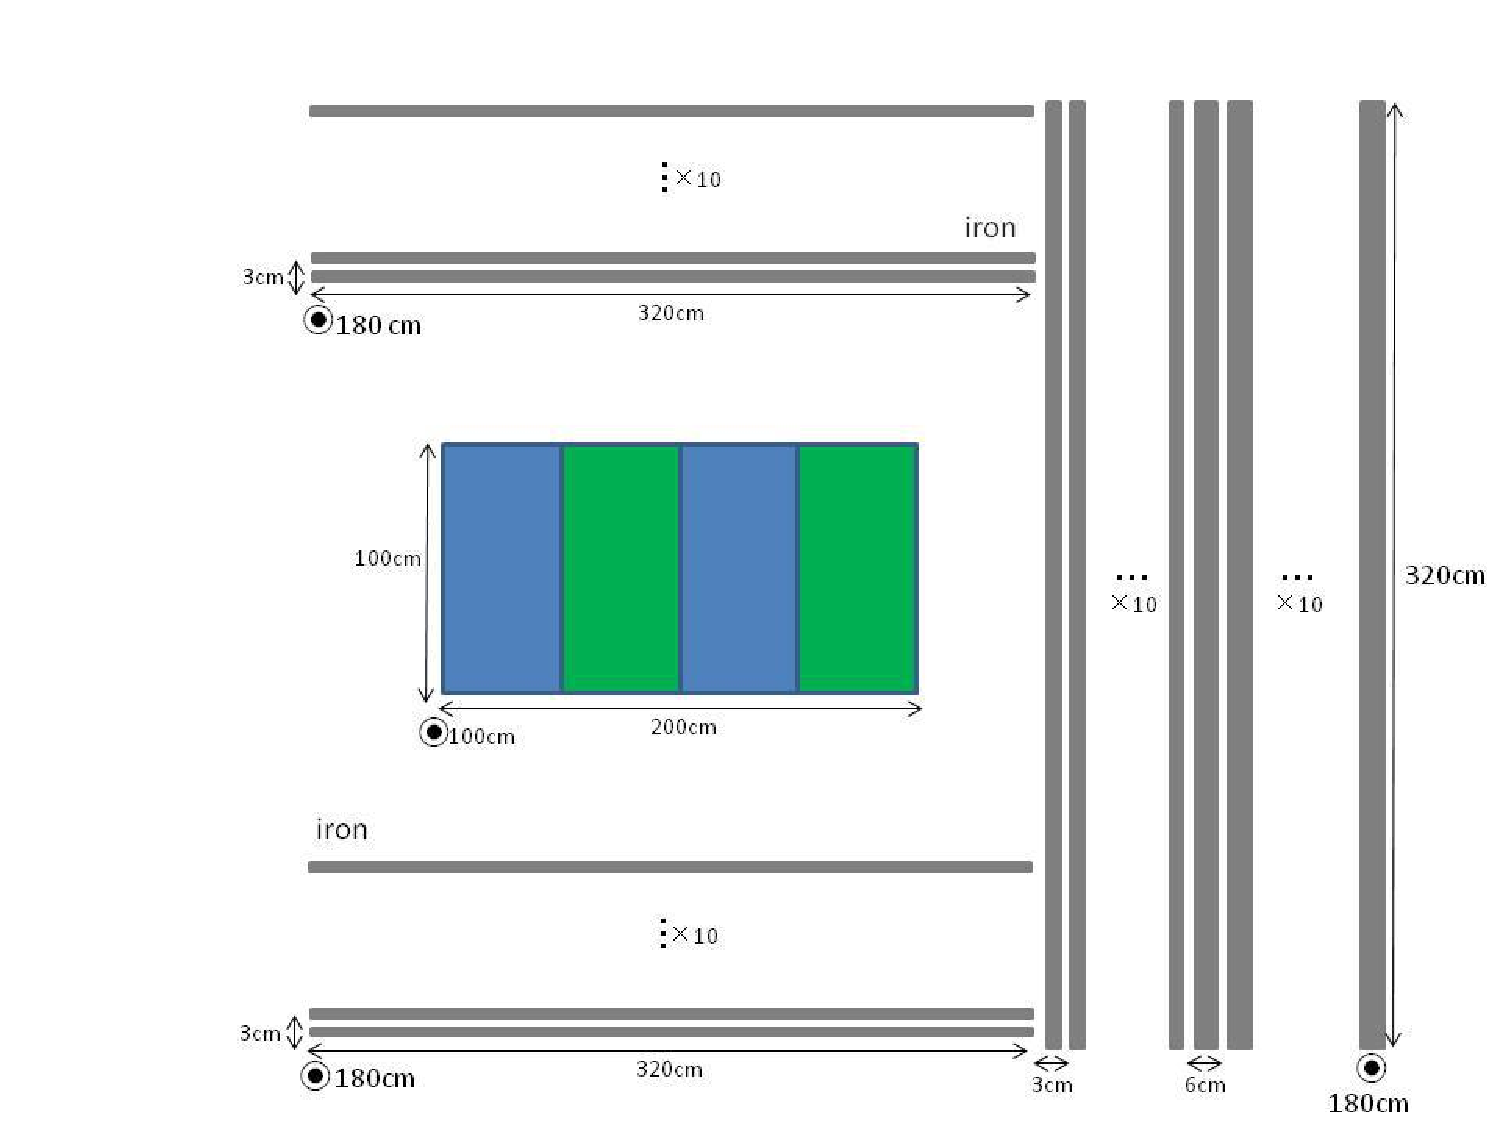
\includegraphics[width=0.8\linewidth]{fig/wagasci_mc_geometry.pdf}
% \includegraphics[width=0.8\linewidth]{fig/all_detector2.pdf}
\end{center}
\caption{
Geometry of the detectors in the Monte Carlo simulation.}
\label{fig:wagasci_mc_geometry}
\end{figure}

\begin{figure}[tbh]
\begin{center}
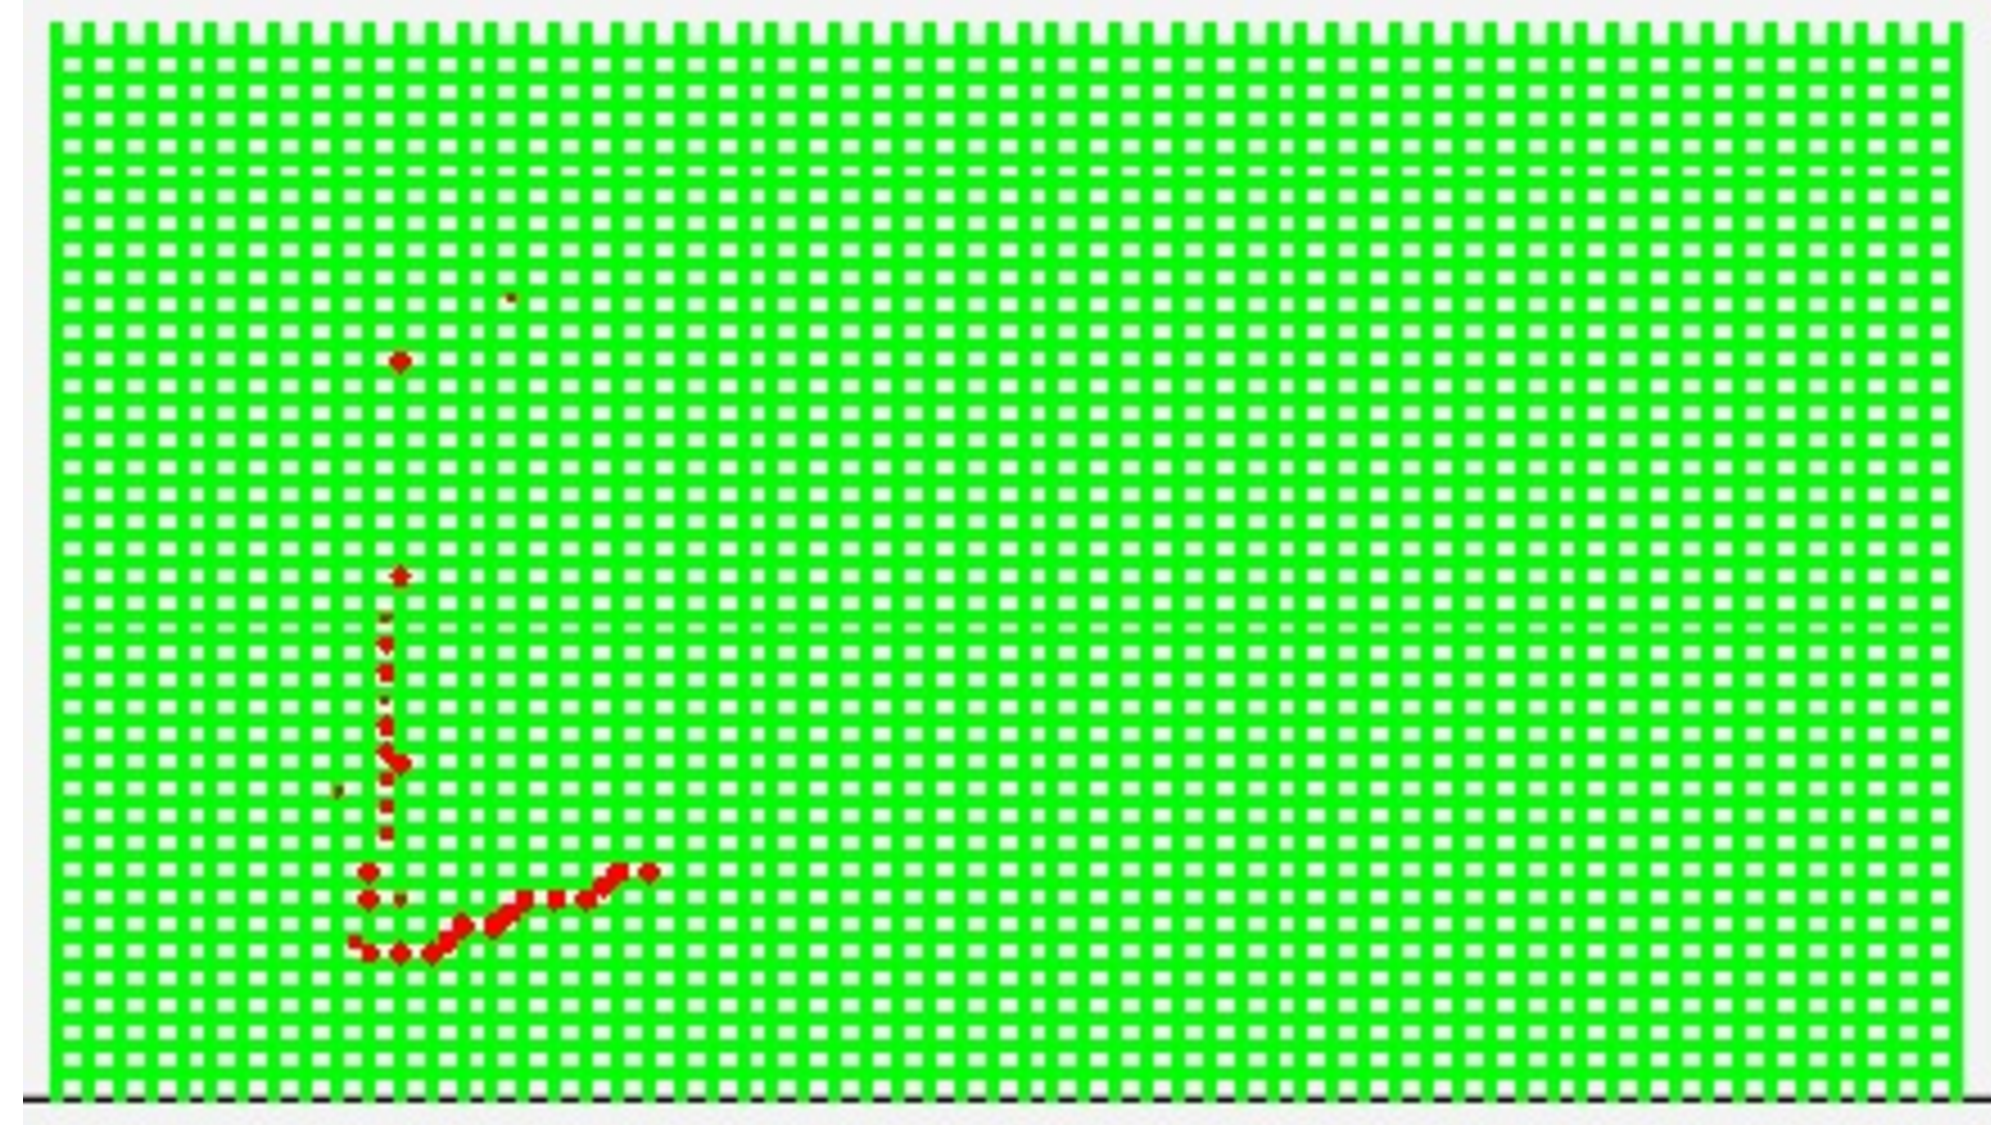
\includegraphics[width=0.8\linewidth]{fig/wagasci_event_display.pdf}
% \includegraphics[width=0.8\linewidth]{fig/all_detector2.pdf}
\end{center}
\caption{
An event display of MC event in Wagasci detectors. Green lines are scintillators and red circles are the hit channels.}
\label{fig:wagasci_mc_geometry}
\end{figure}

% In order to estimate backgrounds from neutrino interactions in the wall and floor of the experimental hall, the geometry of the experimental hall is implemented in the GEANT4-based detector simulation.


\subsubsection{Response of detector components}
The energy deposit inside the scintillator is converted into the number of photons. 
The effects of collection and attenuation of the light in the scintillator and the WLS fiber are simulated, and the MPPC response is also taken into account. 
The light yield is smeared according to statistical fluctuations and electrical noise.


\subsection{Track reconstruction}
To select neutrino interaction from the hit patterns, a track reconstruction algorithm is developed.
The flow of the track reconstruction is as follows.
\begin{enumerate}
\item Two-dimensional track reconstruction in each sub-detectors
\item Track matching among the sub-detectors
\item Three -dimensional track reconstruction
\end{enumerate}

Add explanation about two-dim reco, track matching and three-dim reco here.


\subsection{Event selection}

First, the events with the track which starts in 5 cm from the wall of the Wagasci module are rejected to remove the background from the outside.
% as shown in Fig. \ref{fig:fv_cut}.

% \begin{figure}[tbh]
% \begin{center}
%   \begin{subfigure}{0.48\textwidth}
%     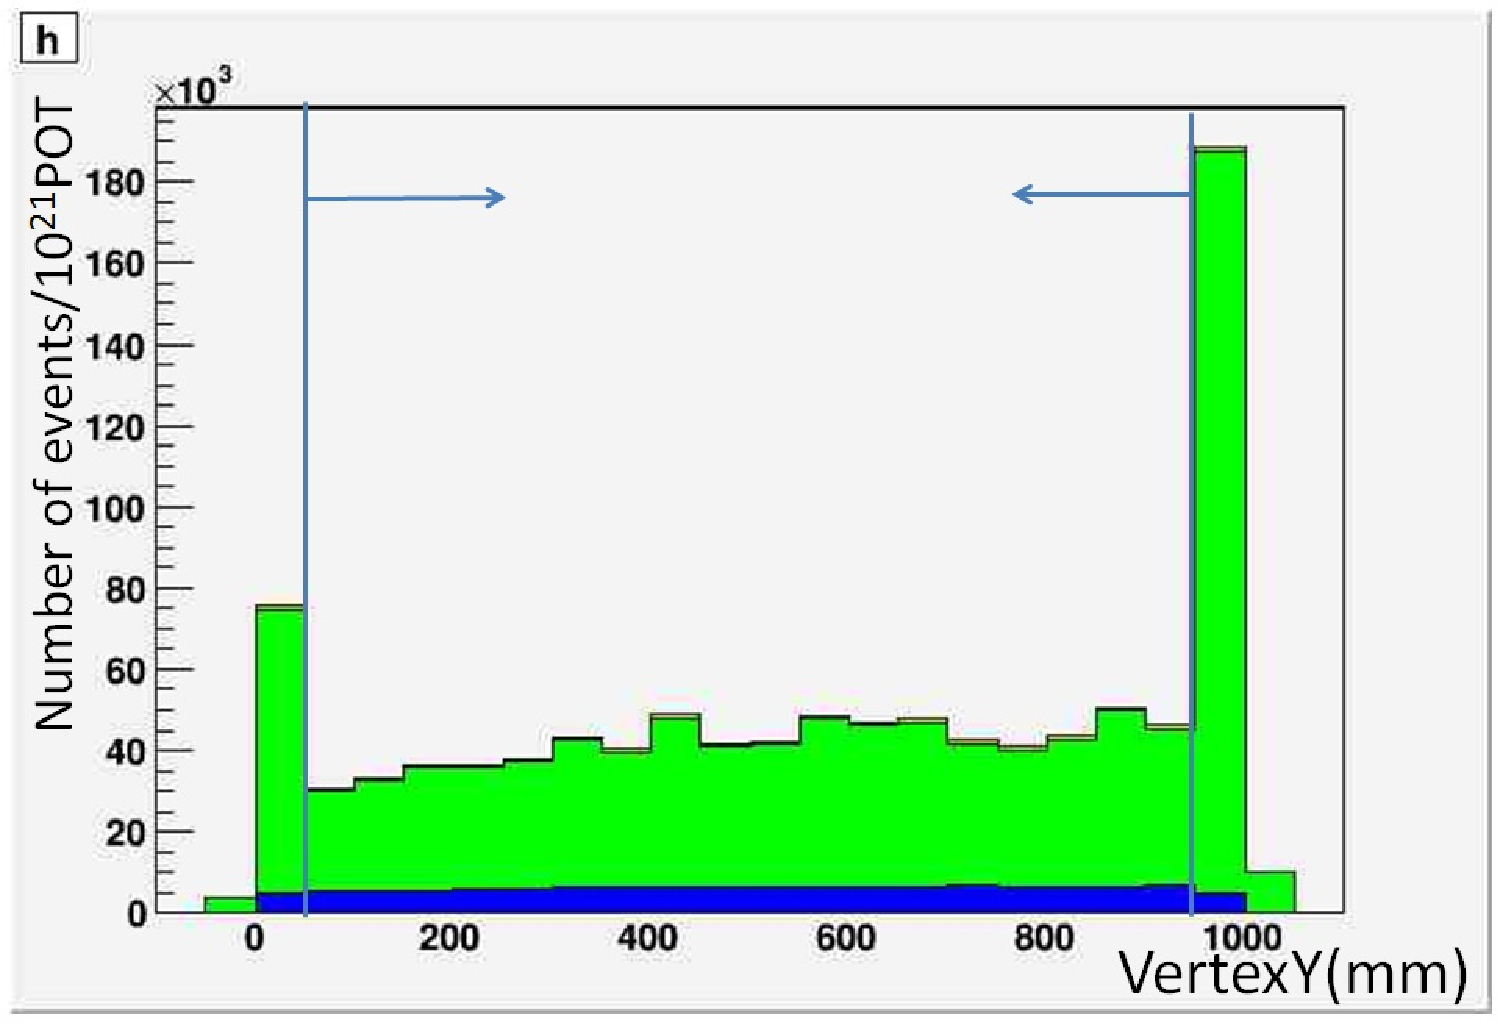
\includegraphics[width=\linewidth]{fig/fv_cut_y.pdf}
%    \end{subfigure}
%  \begin{subfigure}{0.48\textwidth}
%      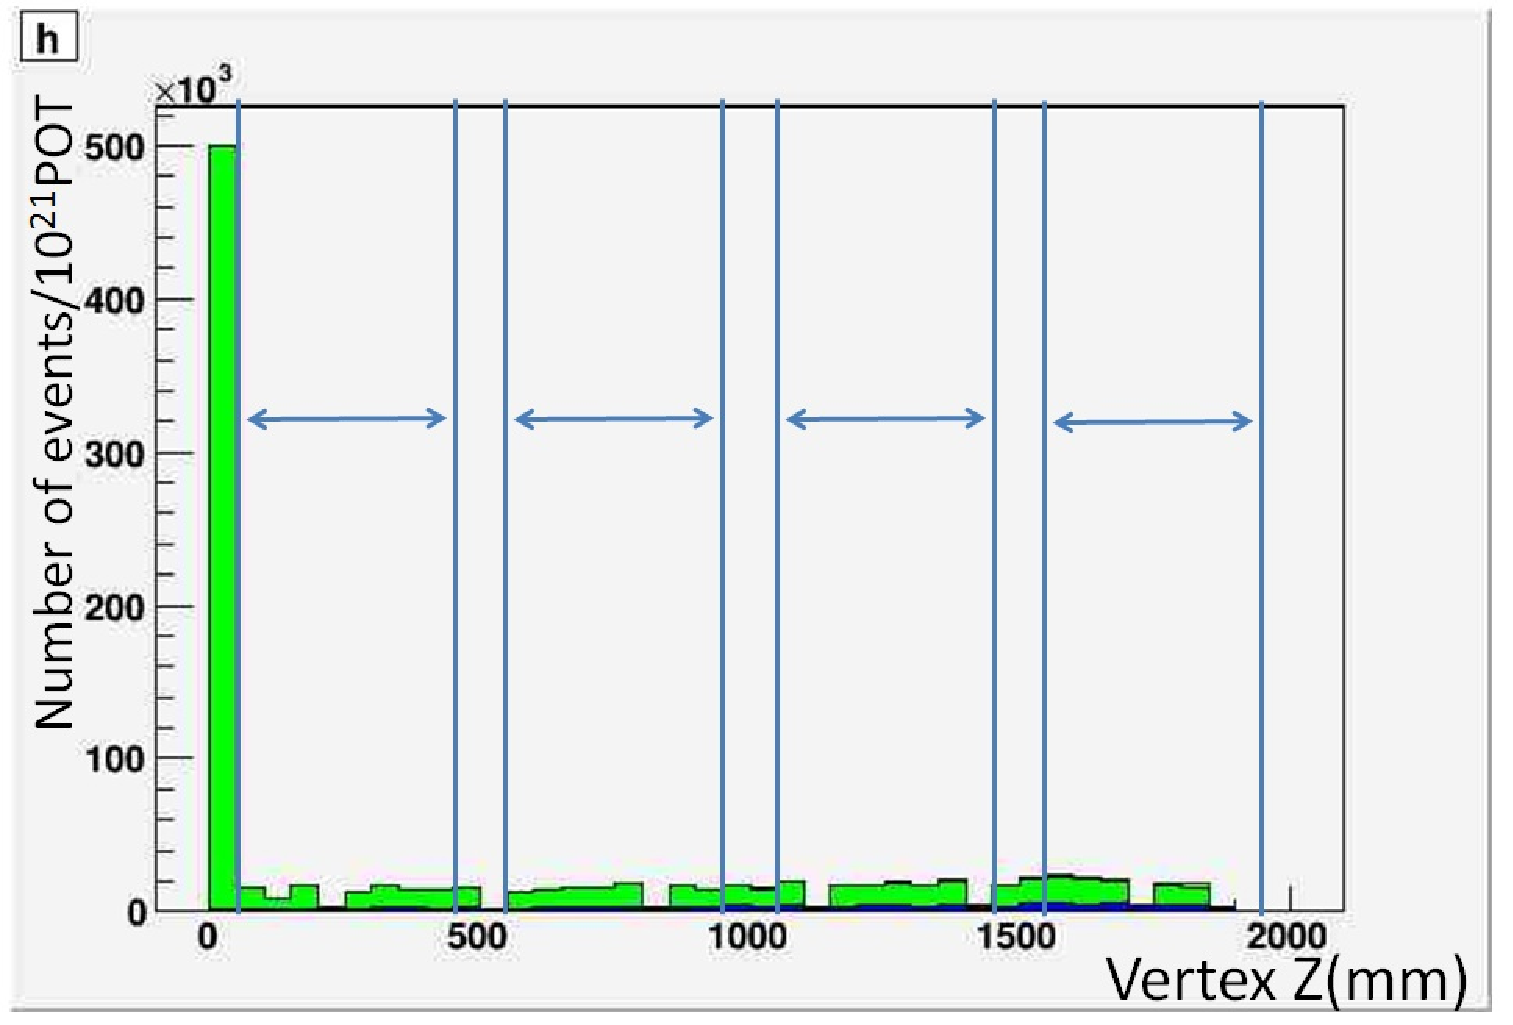
\includegraphics[width=\linewidth]{fig/fv_cut_z.pdf}
%    \end{subfigure}    
%    \end{center}
%  \caption{Event selection with the vertex of the track.
% Blue hist. are events from the Wagasci modules, green hist. are events from the experimental hall, % and yellow hist. are events from the Side-MRD modules and the downstream-MRD.
% }
% \label{fig:fv_cut}
% \end{figure}

Second, to reject backgrounds from NC and neutral particles, the longest tracks are required to penetrate more than one (five) iron plates in Side-MRD modules (Baby-MIND). 
%as shown in Figure \ref{fig:penetrated_iron_plates_cut}.
Then, in order to measure muon momentum, the longest tracks are required to stop in MRDs (Side-MRD modules and Baby-MIND) or penetrate all iron plates.

% \begin{figure}[tbh]
%  \begin{center}
%   \begin{subfigure}{0.48\textwidth}
%      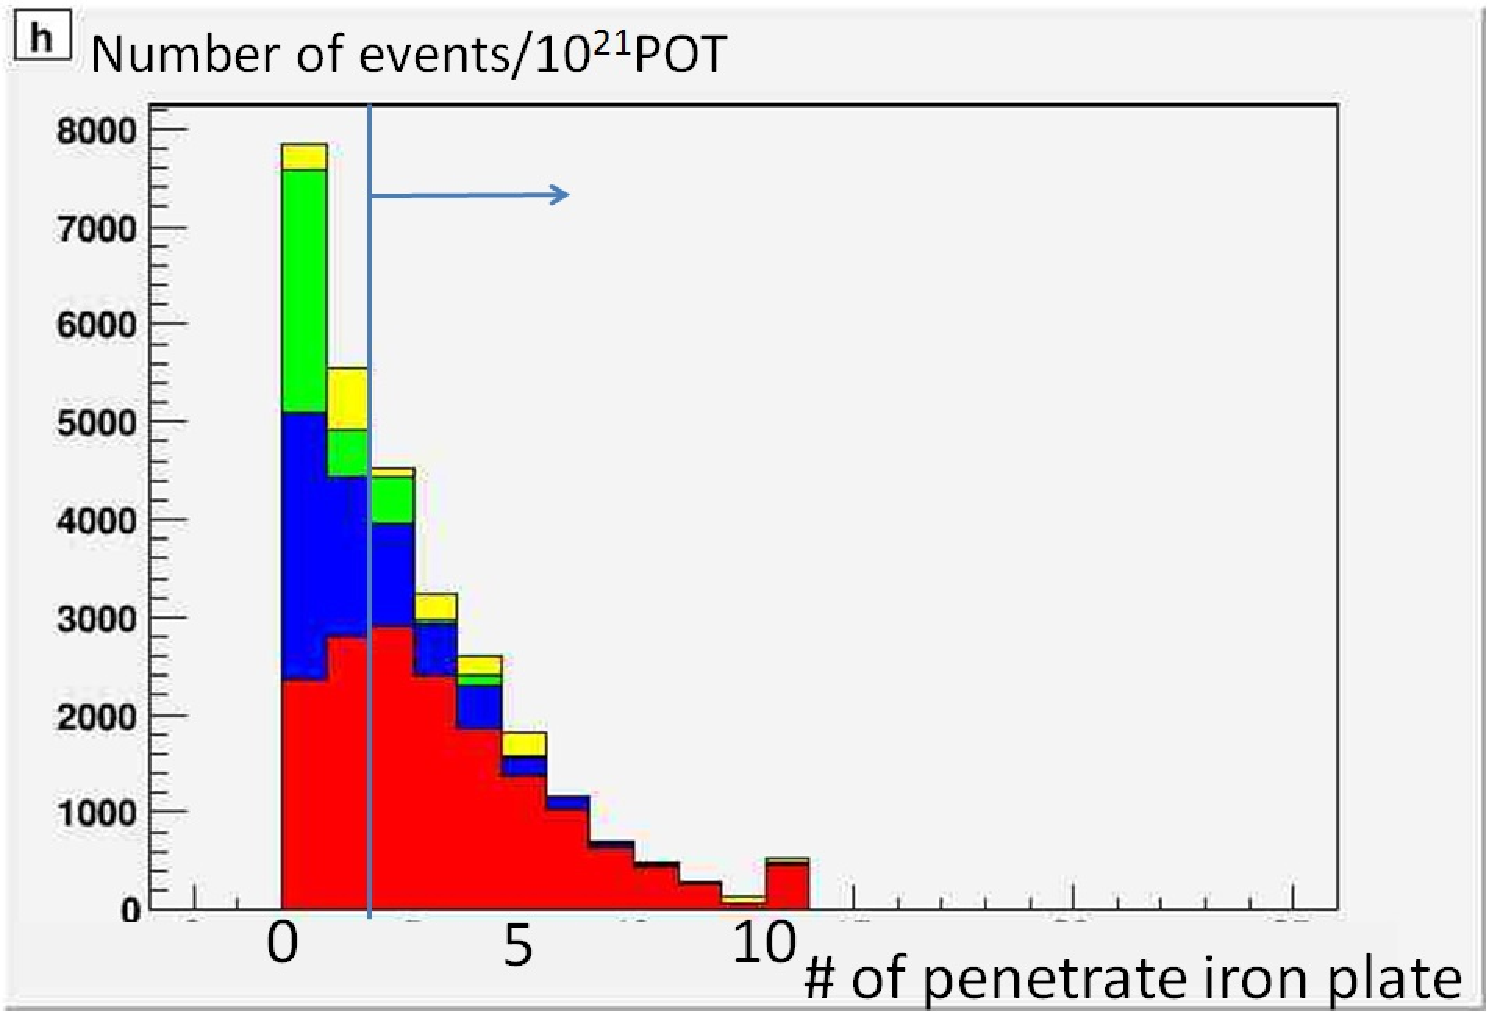
\includegraphics[width=\linewidth]{fig/penetrated_iron_plates_cut_sidemrd.pdf}
%     \end{subfigure}
%   \begin{subfigure}{0.48\textwidth}
%     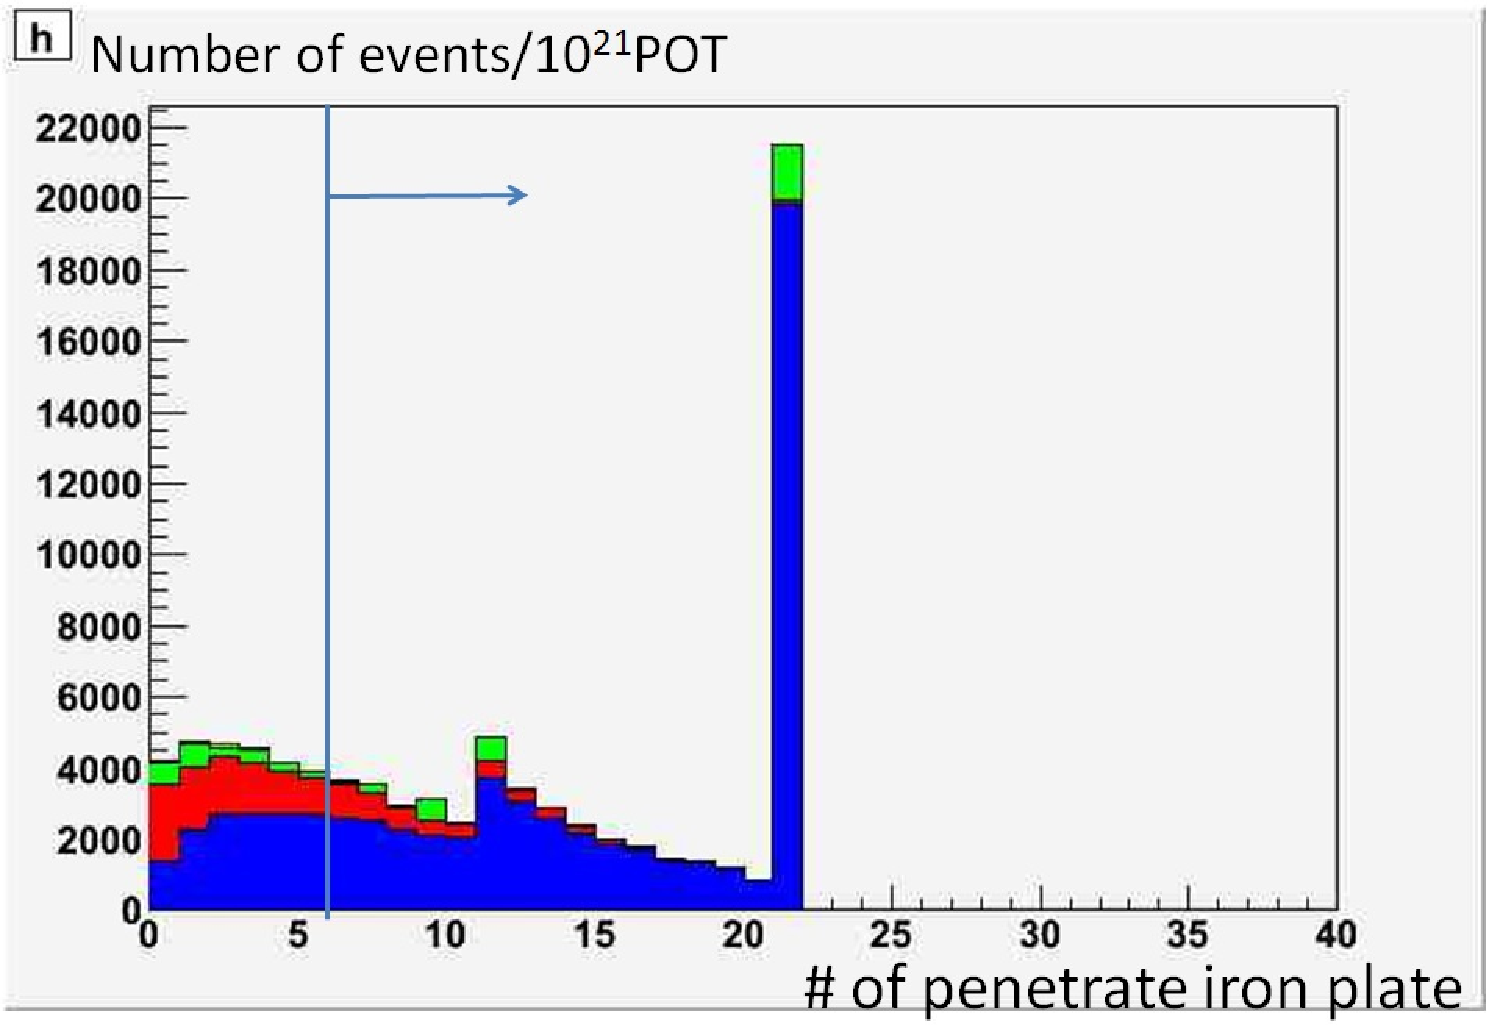
\includegraphics[width=\linewidth]{fig/penetrated_iron_plates_cut_babymind.pdf}
%     \end{subfigure}    
%     \end{center}
%   \caption{
% Event selection with the number of the penetrated iron plates in the Side-MRD modules (left) and the Baby-MIIND (right).
% Blue and red hist. are events from the Wagasci modules, green hist. are events from the experimental hall, and yellow hist. are events from the Side-MRD modules and the Baby-MIND.
% }
% \label{fig:penetrated_iron_plates_cut}
% \end{figure}

% \subsection{Selected events}


Table \ref{tab:expected_num_events_neutrino_beam} and \ref{tab:expected_num_events_antineutrino_beam}  show numbers of the selected events in one water-in Wagasci module after each event election in neutrino-mode and antineutrino-mode respectively.
As for the neutrino-mode, $2.12 \times 10^{4}$ CC events are expected with $1 \times 10^{21}$  POT, and the purity is 81.3 \%.
The main background for the neutrino-mode is the neutrino interactions in the scintillators inside the Wagasci detector.
As for the antineutrino-mode, $0.83 \times 10^{4}$ CC events are expected with $1 \times 10^{21}$  POT, and the purity is 62.0 \%.
The main background for the antineutrino-mode is the wrong sign contamination from $\nu_{\mu}$ events and the antineutrino interactions in the scintillators inside the Wagasci detector.

\begin{table}[htb]
  \begin{center}
    \caption{Expected number of the neutrino-candidate events in one water-in Wagasci module with 1$\times 10^{21}$ POT in neutrino-mode.}
    \begin{tabular}{c|ccc|c} \hline
Cut   & CC & NC & Scinti Bkg. & Total \\ \hline
Reconstructed & 18093.2 & 699.7 & 4698.3 & 23491.2 \\
FV & 15150.8 & 588.4 & 3934.8 & 19673.9 \\
Pene. iron & 11264.3 & 237.3 & 2875.4 & 14377.0 \\
Stop/Penetrate MRDs & 8478.2 & 214.0 & 2173.1 & 10865.2 \\ \hline
after all cuts & 78.0 \% & 2.0 \% & 20.0 \% & 100 \% \\
\hline
    \end{tabular}
    \label{tab:expected_num_events_neutrino_beam}
  \end{center}
\end{table}

\begin{table}[htb]
  \begin{center}
    \caption{Expected number of the antineutrino-candidate events in one water-in Wagasci module with 1$\times 10^{21}$ POT in antineutrino-mode.}
    \begin{tabular}{c|cccc|c} \hline
 Cut   & CC & NC & Scinti Bkg. & Wrong sign bkg & Total \\ \hline
Reconstructed & 6499.7 & 107.3 & 2234.4 & 2330.8 & 11172.1 \\ 
FV & 5457.9 & 89.3 & 1873.5 & 1946.6 & 9367.1 \\ 
Pene. iron & 4172.3 & 30.8 & 1440.9 & 1560.6 & 7204.6 \\ 
Stop/Penetrate MRDs & 3331.5 & 28.5 & 1120.3 & 1121.2 & 5601.5 \\ \hline
after all cuts & 59.5 \% & 0.5 \% & 20.0 \% &  20.0 \% & 100 \% \\
\hline
    \end{tabular}
    \label{tab:expected_num_events_antineutrino_beam}
  \end{center}
\end{table}

\begin{table}[htb]
  \begin{center}
    \caption{Expected number of the charged-current events in one water-in Wagasci module after the event selections with 1$\times 10^{21}$ POT in neutrino-mode with a classification based on interactions at a vertex.}
    \begin{tabular}{cccc|c} \hline
CCQE & MEC & CCRes & CCDIS & Total \\ \hline
3716.3 & 747.0 & 2081.3 & 1933.7 & 8478.3 \\
\hline
    \end{tabular}
    \label{tab:expected_num_cc_events_neutrino_beam}
  \end{center}
\end{table}

\begin{table}[htb]
  \begin{center}
    \caption{Expected number of the charged-current events in one water-in Wagasci module after the event selections with 1$\times 10^{21}$ POT in neutrino-mode with a classification based on particles after final state interactions.}
    \begin{tabular}{ccc|c} \hline
CC0$\pi$ & CC1$\pi$ & CCn$\pi$  & Total \\ \hline
5423.1 & 1684.3 &  & \\
\hline
    \end{tabular}
    \label{tab:expected_num_ccfsi_events_neutrino_beam}
  \end{center}
\end{table}

\begin{table}[htb]
  \begin{center}
    \caption{Expected number of the charged-current events in one water-in Wagasci module after the event selections with 1$\times 10^{21}$ POT in antineutrino-mode with a classification based on interactions at a vertex.}
    \begin{tabular}{cccc|c} \hline
CCQE & MEC & CCRes & CCDIS & Total \\ \hline
2522.0 & 362.8 & 765.8 & 770.6 & 4421.2 \\
\hline
    \end{tabular}
    \label{tab:expected_num_cc_events_antineutrino_beam}
  \end{center}
\end{table}

\begin{table}[htb]
  \begin{center}
    \caption{Expected number of the charged-current events in one water-in Wagasci module after the event selections with 1$\times 10^{21}$ POT in antineutrino-mode with a classification based on  particles after final state interactions.}
    \begin{tabular}{ccc|c} \hline
CC0$\pi$ & CC1$\pi$ & CCn$\pi$  & Total \\ \hline
2529.3 & 520.0 &  & \\
\hline
    \end{tabular}
    \label{tab:expected_num_ccfsi_events_antineutrino_beam}
  \end{center}
\end{table}


% Table \ref{tab:expected_num_events_neutrino_beam} shows numbers of the selected events after each event election.
% $2.41 \times 10^{4}$ CC events are expected with $1 \times 10^{21}$  POT in neutrino-mode, and the purity is 75.5 \%.
% The main background is the neutrino interaction in the scintillators inside the Wagasci detector.
% 
% \begin{table}[htb]
%   \begin{center}
%     \caption{Expected number of the neutrino-candidate events in two Wagasci modules after the event selections with 1$\times 10^{21}$ POT in neutrino-mode.}
%     \begin{tabular}{c|cccc|c} \hline
%       Cut & CC & NC & BG (Scinti.) & BG (outside) \\ \hline
%      Track reconst. & $6.27 \times 10^{4}$  & $3.61\times10^{3}$ & $1.62 \times10^{4}$ & $1.04 \times 10^{6}$ & $1.12 \times 10^{6}$ \\
%      Fiducial & $3.95 \times 10^{4}$  & $1.75 \times10^{3}$ & $9.71 \times10^{3}$ & $7.32 \times 10^{3}$ & $5.55 \times 10^{4}$ \\
%      Penetrated iron & $3.02 \times 10^{4}$  & $9.12 \times10^{2}$ & $7.67 \times10^{3}$ & $2.04 \times 10^{3}$ & $4.00 \times 10^{4}$ \\
%      Stop in MRDs & $2.41 \times 10^{4}$  & $8.65 \times10^{2}$ & $6.19 \times10^{3}$ & $1.64 \times 10^{3}$ & $3.19 \times 10^{4}$ \\ \hline
%     after all cuts & 75.5 \% & 2.71 \% & 19.4 \% & 5.14 \% & 100 \% \\
%     \hline
%     \end{tabular}
%     \label{tab:expected_num_events_neutrino_beam}
%   \end{center}
% \end{table}


% Figure \ref{fig:angle_allcut_neutrino} shows the reconstructed angles of the longest tracks in the selected events.
%Figure \ref{fig:angle_resolution_neutrino} shows differences between true angles and the reconstructed angles of the longest tracks in the selected events, and the angle resolution is $\sim$3 degrees.
%
%\begin{figure}[tbh]
%\begin{center}
%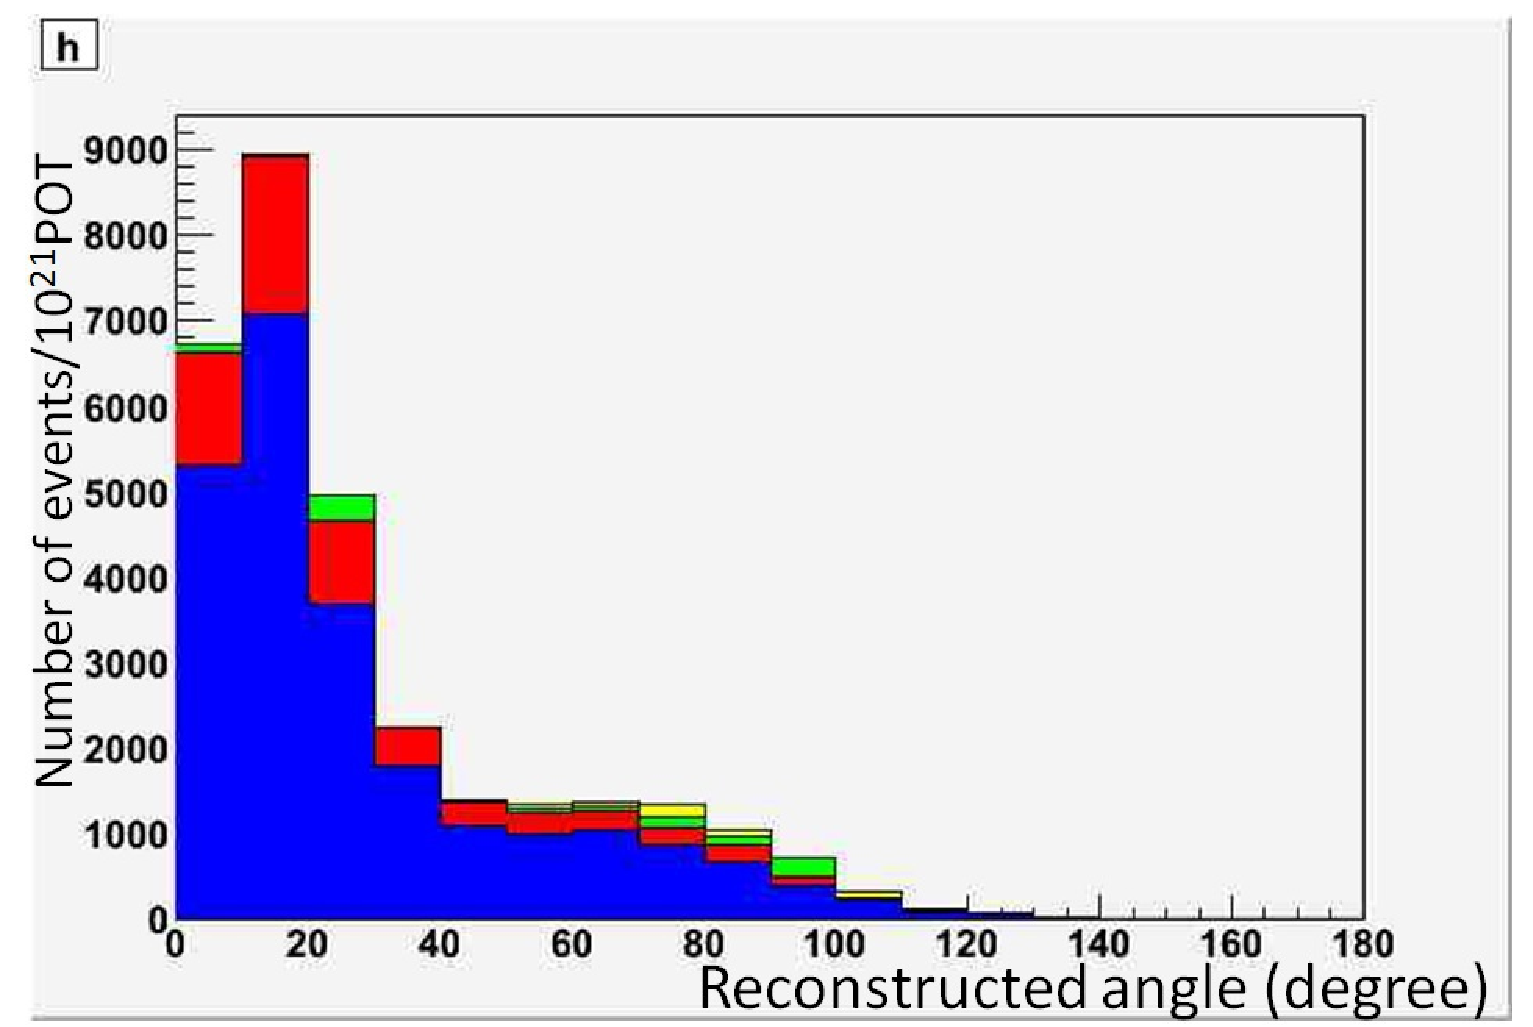
\includegraphics[width=0.8\linewidth]{fig/angle_allcut_neutrino.pdf}
% \includegraphics[width=0.8\linewidth]{fig/all_detector2.pdf}
%\end{center}
%\caption{
%The reconstructed angles of the longest tracks in the selected events.
%Blue and red hist. are events from water and scintillators in the Wagasci modules, green hist. are events from the experimental hall, and yellow hist. are events from the Side-MRD modules and the Baby-MIND.
%}
%\label{fig:angle_allcut_neutrino}
%\end{figure}

%\begin{figure}[tbh]
%\begin{center}
%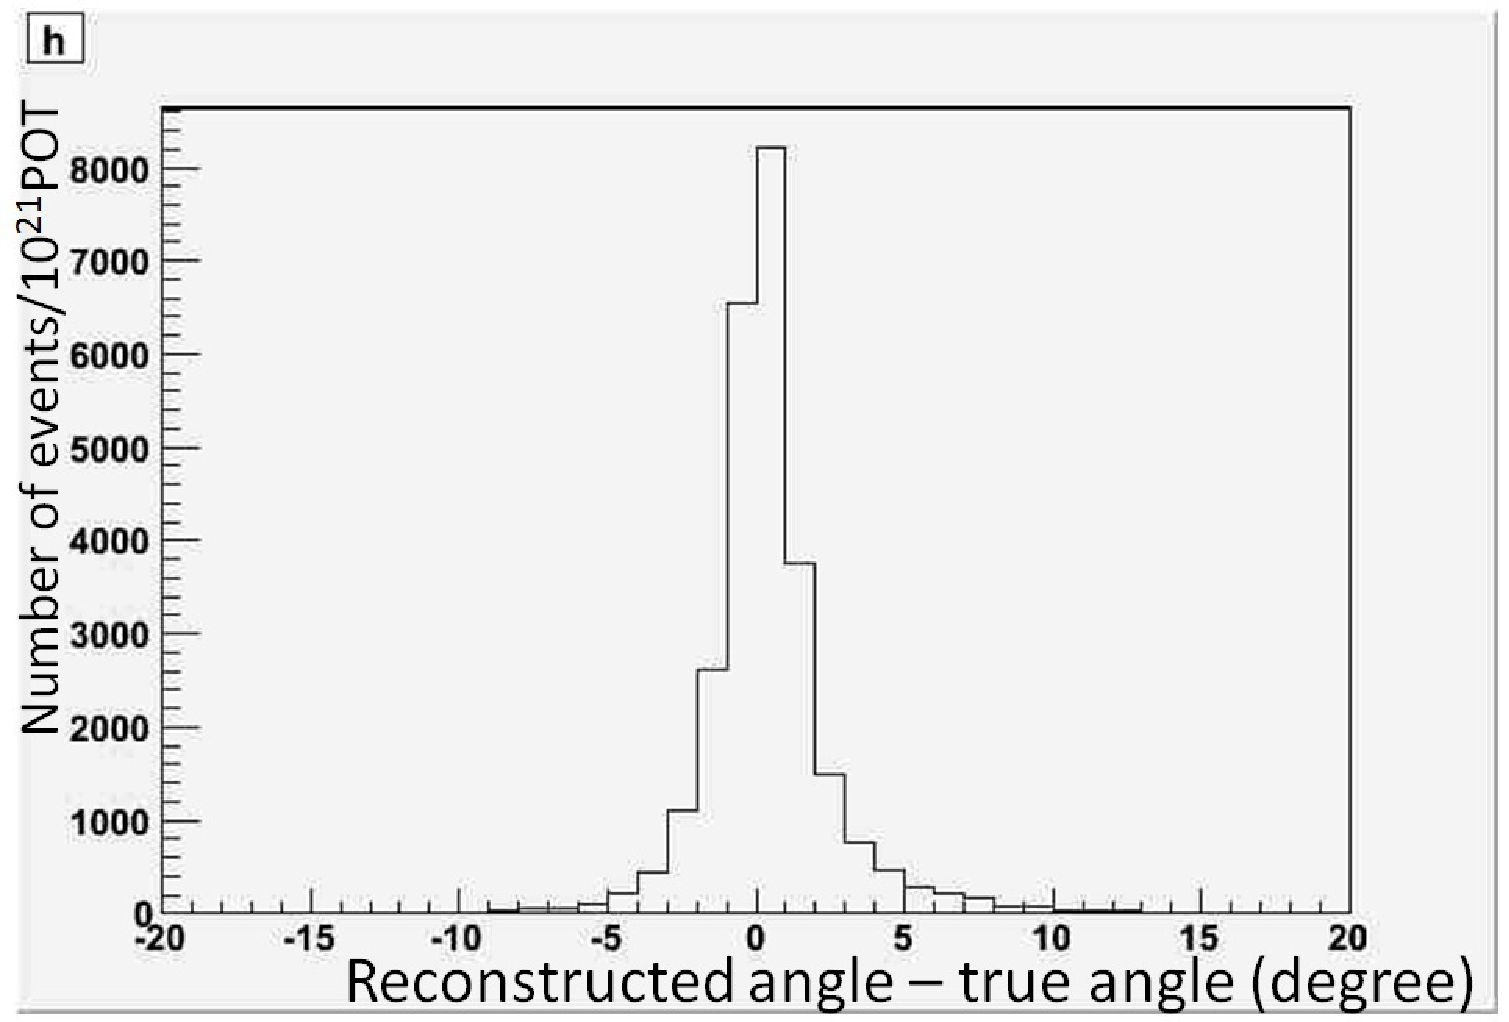
\includegraphics[width=0.8\linewidth]{fig/angle_resolution_neutrino.pdf}
% \includegraphics[width=0.8\linewidth]{fig/all_detector2.pdf}
%\end{center}
%\caption{
%Differences between true angles and the reconstructed angles of the longest tracks in the selected events.
%}
%\label{fig:angle_resolution_neutrino}
%\end{figure}

Figure \ref{fig:angle_allcut_neutrino} and \ref{fig:angle_allcut_antineutrino} show the reconstructed angles of the longest tracks in the selected events in the neutrino-mode and the anti-neutrino mode respectively.

\begin{figure}[tbh]
\begin{center}
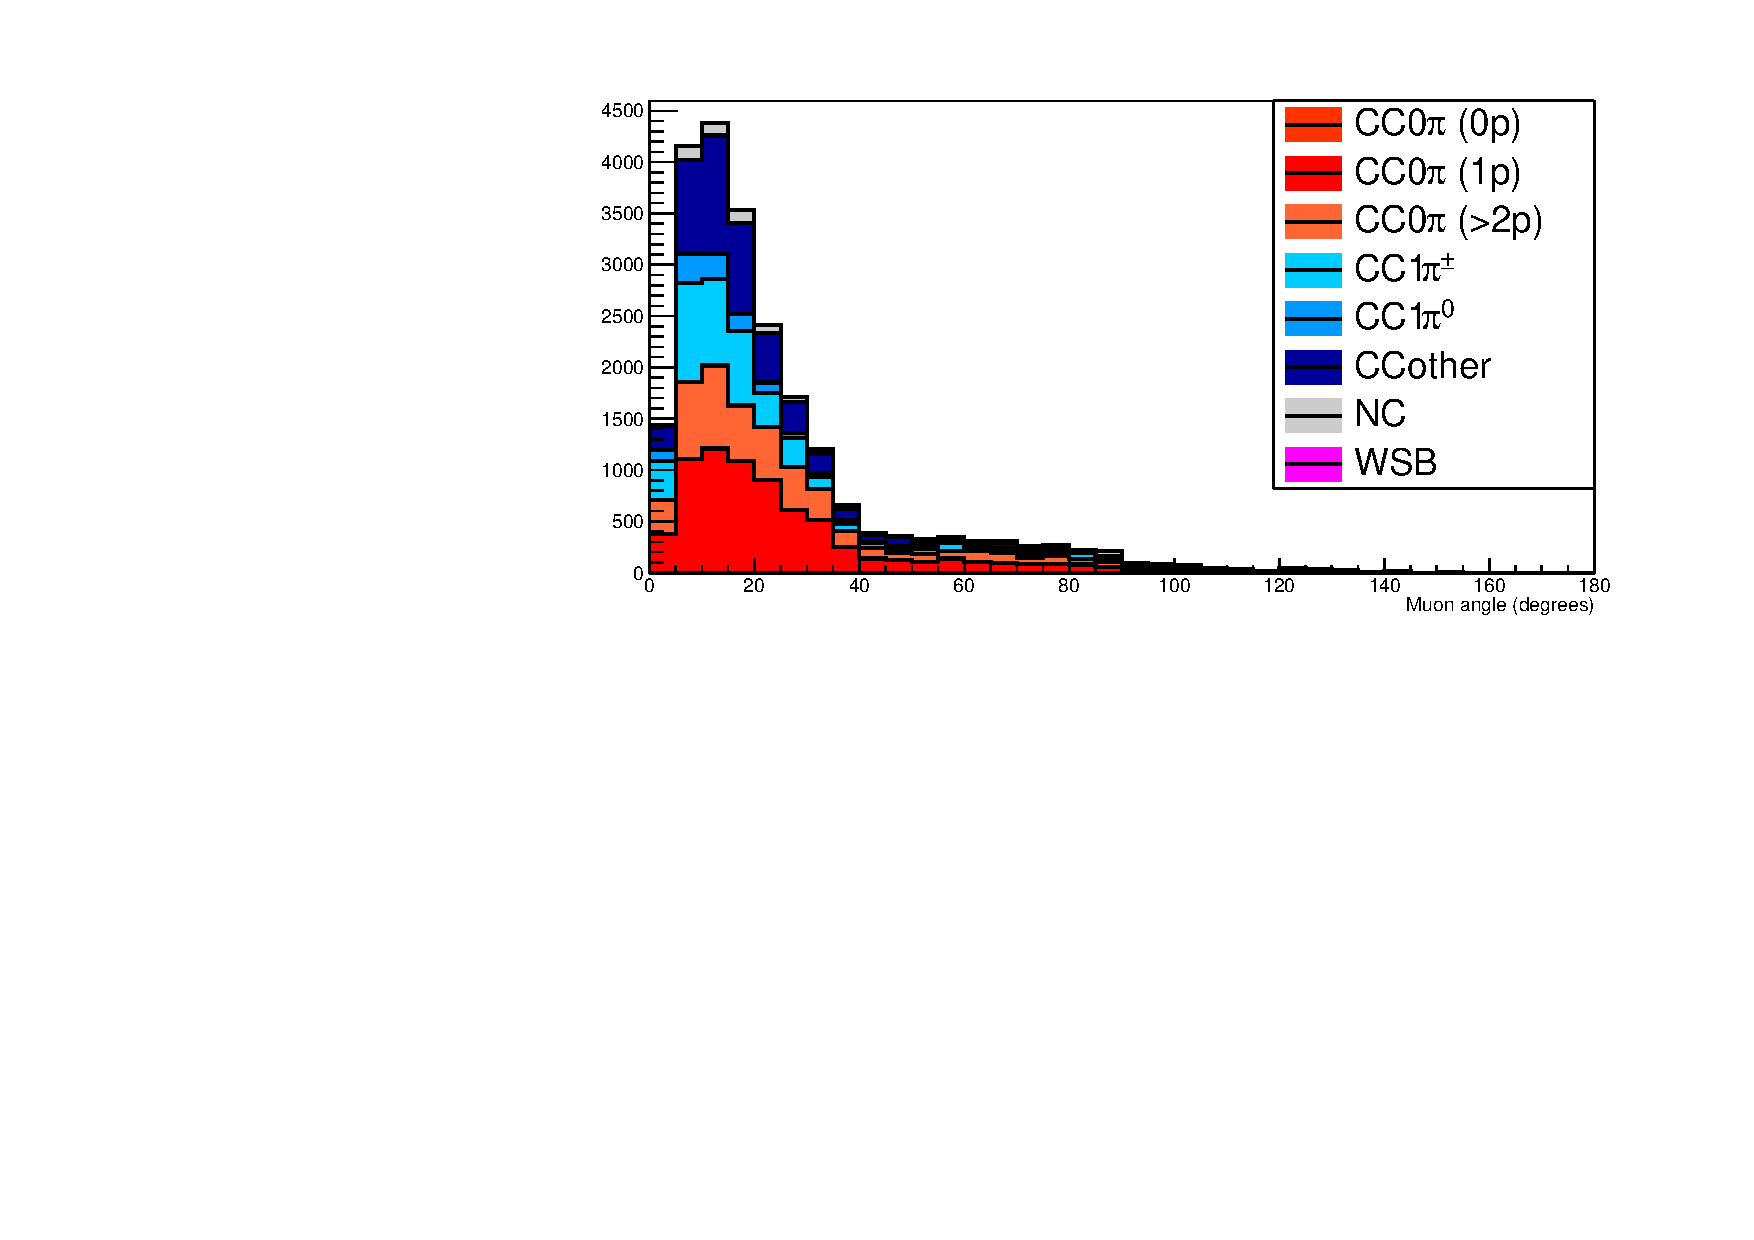
\includegraphics[width=0.5\linewidth, angle=270]{fig/FHCMuonAngle_StoppedOrThroughGoing.pdf}
% \includegraphics[width=0.8\linewidth]{fig/all_detector2.pdf}
\end{center}
\caption{
The reconstructed angles of the longest tracks in the selected events in the neutrino-mode.
% Blue and red hist. are events from water and scintillators in the Wagasci modules, green hist. are events from the experimental hall, and yellow hist. are events from the Side-MRD modules and the Baby-MIND.
}
\label{fig:angle_allcut_neutrino}
\end{figure}

\begin{figure}[tbh]
\begin{center}
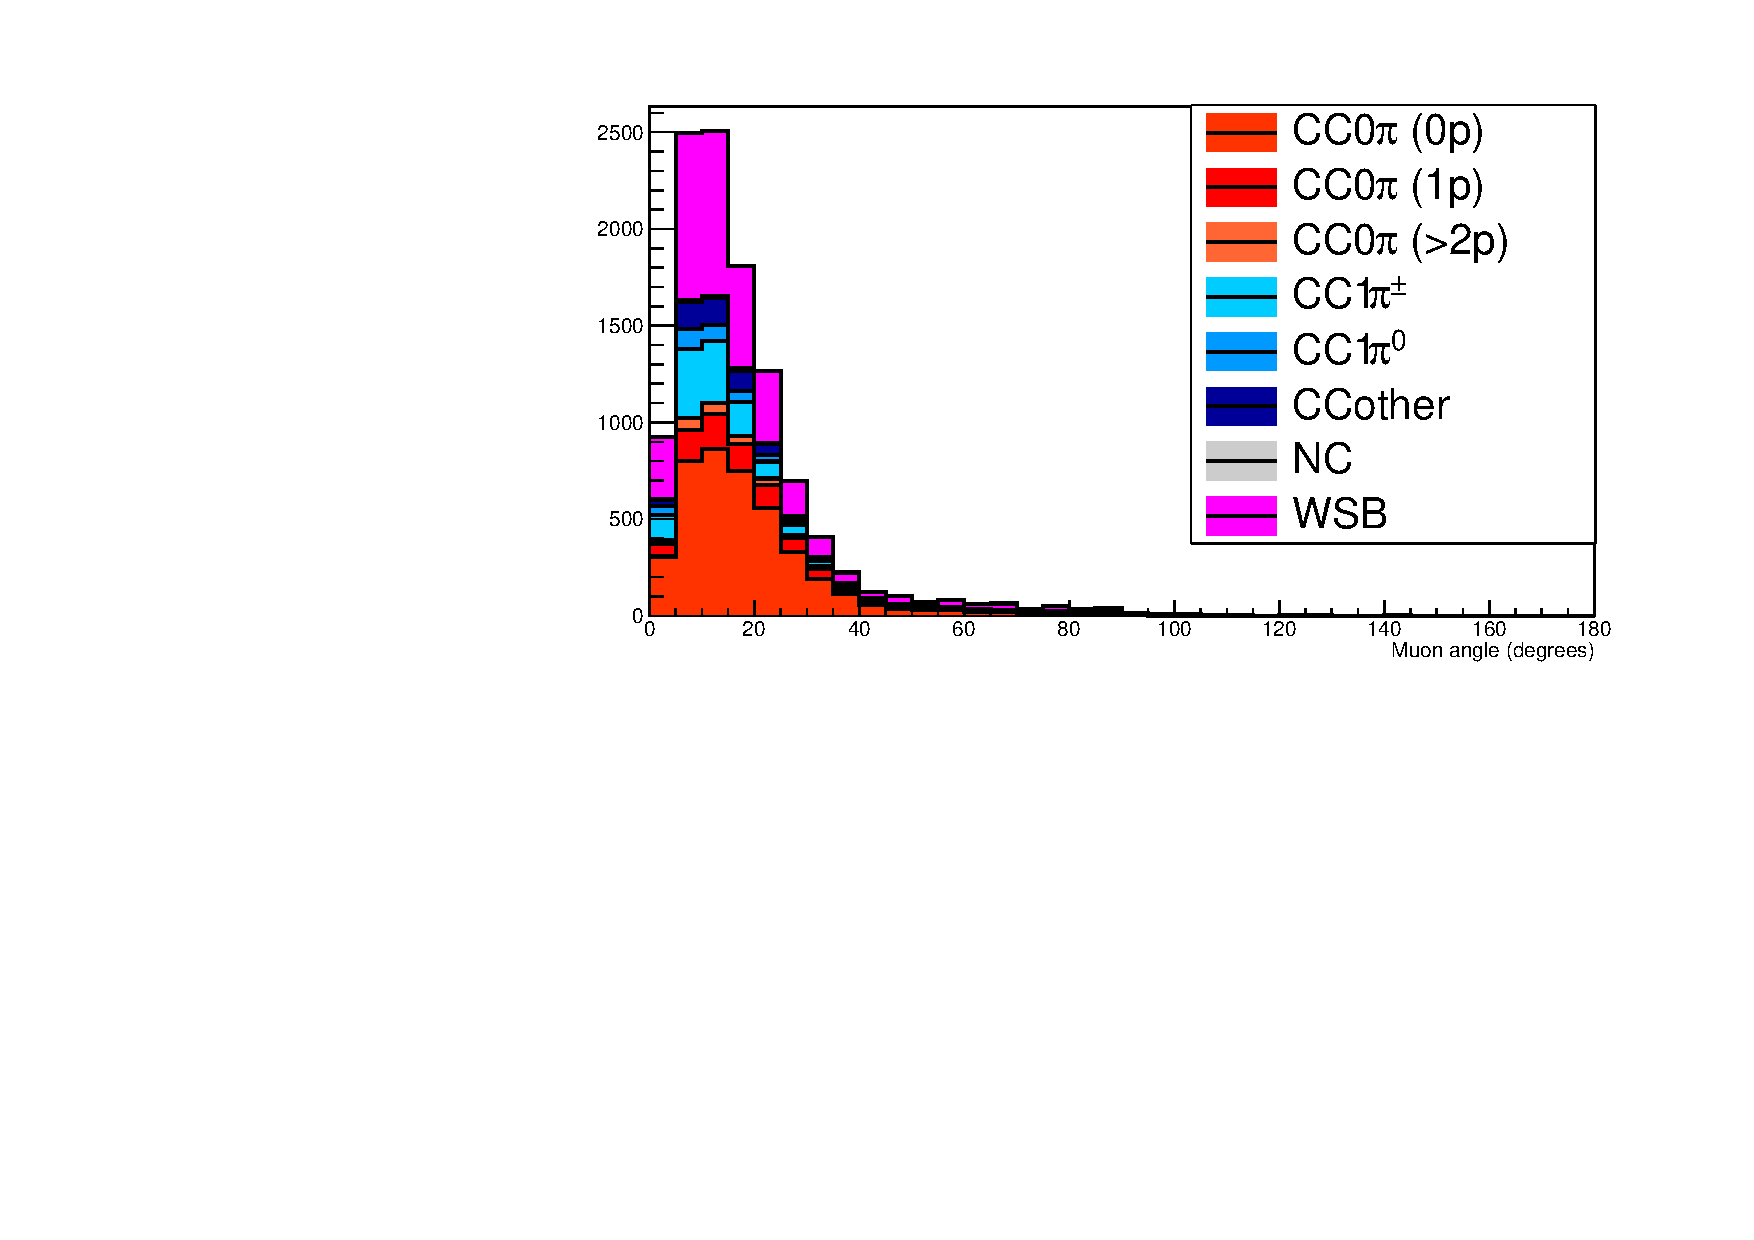
\includegraphics[width=0.5\linewidth, angle=270]{fig/RHCMuonAngle_StoppedOrThroughGoing.pdf}
% \includegraphics[width=0.8\linewidth]{fig/all_detector2.pdf}
\end{center}
\caption{
The reconstructed angles of the longest tracks in the selected events in the antineutrino-mode.
% Blue and red hist. are events from water and scintillators in the Wagasci modules, green hist. are events from the experimental hall, and yellow hist. are events from the Side-MRD modules and the Baby-MIND.
}
\label{fig:angle_allcut_antineutrino}
\end{figure}


%Figure \ref{fig:endpoint_longest_track_neutrino} shows the iron plane numbers corresponding to the %end points of the longest tracks in the selected events.
%
%\begin{figure}[tbh]
%  \begin{center}
%   \begin{subfigure}{0.48\textwidth}
%     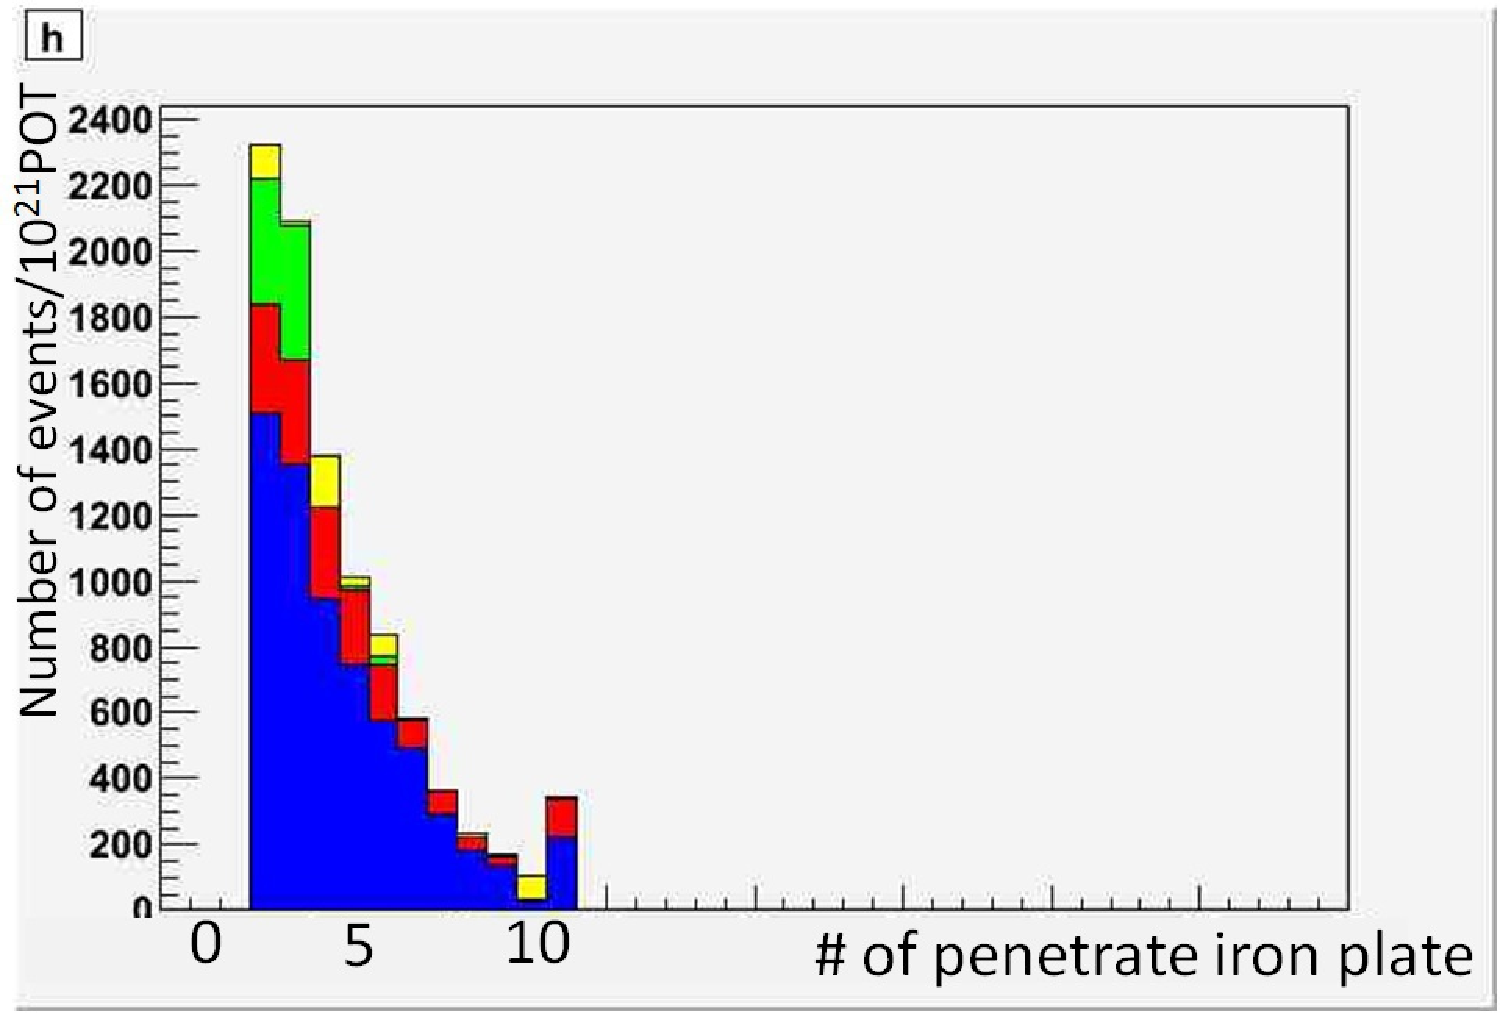
\includegraphics[width=\linewidth]{fig/endpoint_sidemrd_longest_track_neutrino.pdf}
%    \end{subfigure}
%  \begin{subfigure}{0.48\textwidth}
%      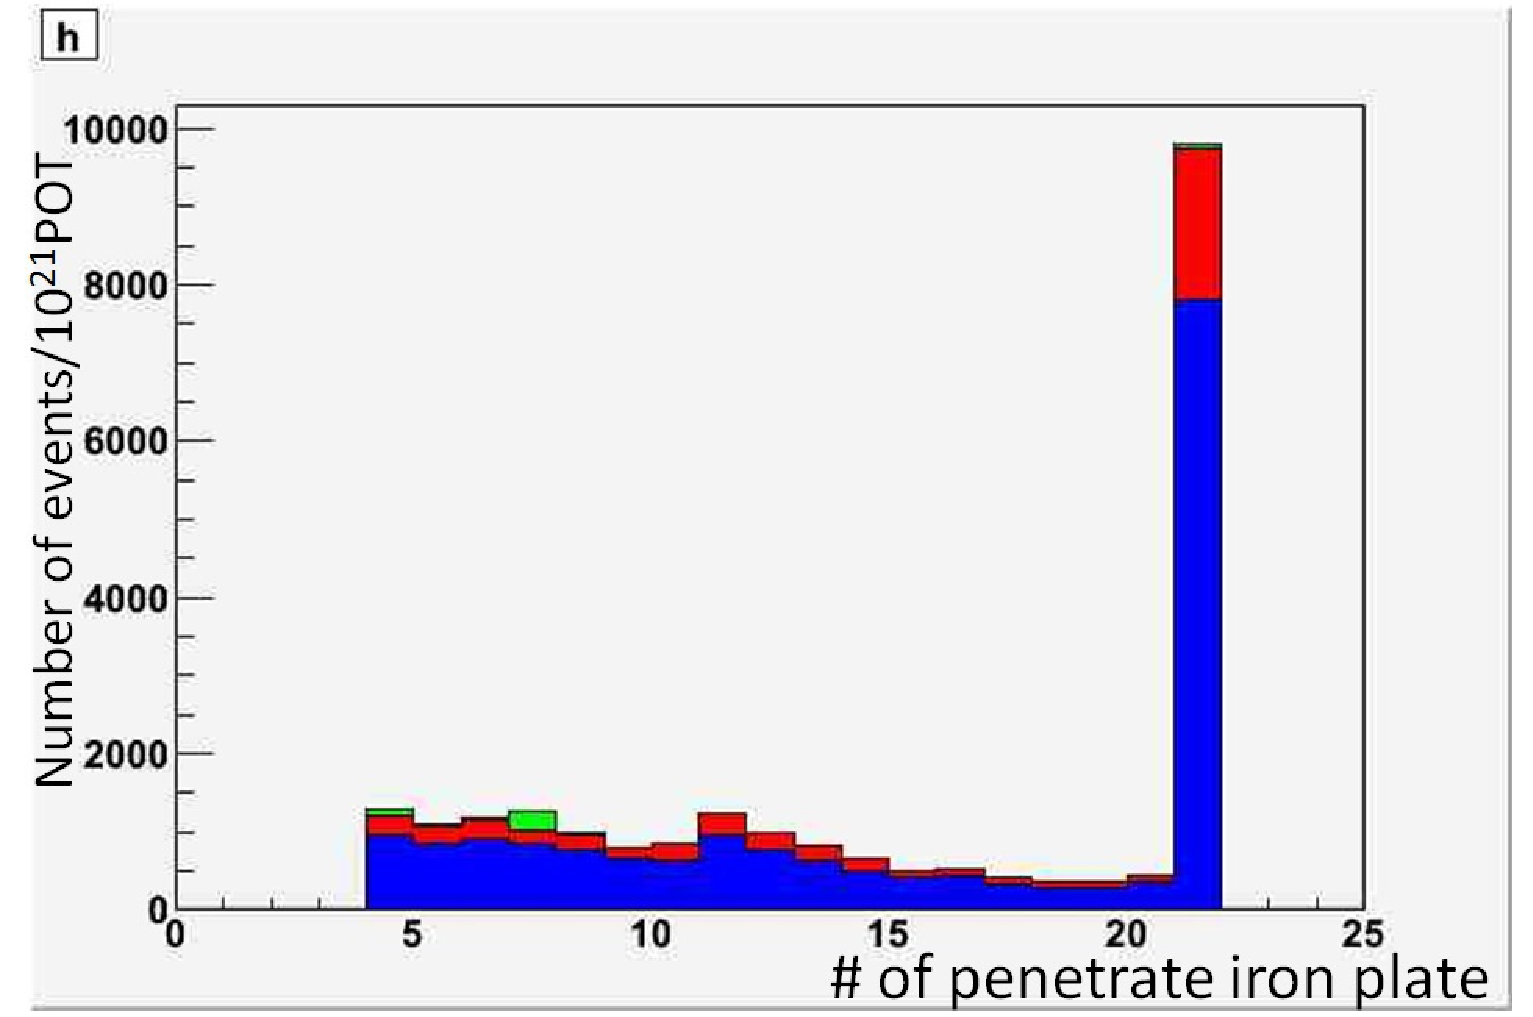
\includegraphics[width=\linewidth]{fig/endpoint_babymind_longest_track_neutrino.pdf}
%    \end{subfigure}    
%    \end{center}
%  \caption{
%Iron plane numbers in Side-MRD (left) and Baby-MIND (right) corresponding to the end points of the longest tracks in the selected events.
%Blue and red hist. are events from water and scintillators in the Wagasci modules, green hist. are events from the experimental hall, and yellow hist. are events from the Side-MRD modules and the Baby-MIND.
%}
%\label{fig:endpoint_longest_track_neutrino}
%\end{figure}


Figure \ref{fig:endpoint_longest_track_neutrino} and \ref{fig:endpoint_longest_track_antineutrino} show the iron plane numbers corresponding to the end points of the longest tracks in the selected events.

\begin{figure}[tbh]
  \begin{center}
   \begin{subfigure}{0.48\textwidth}
     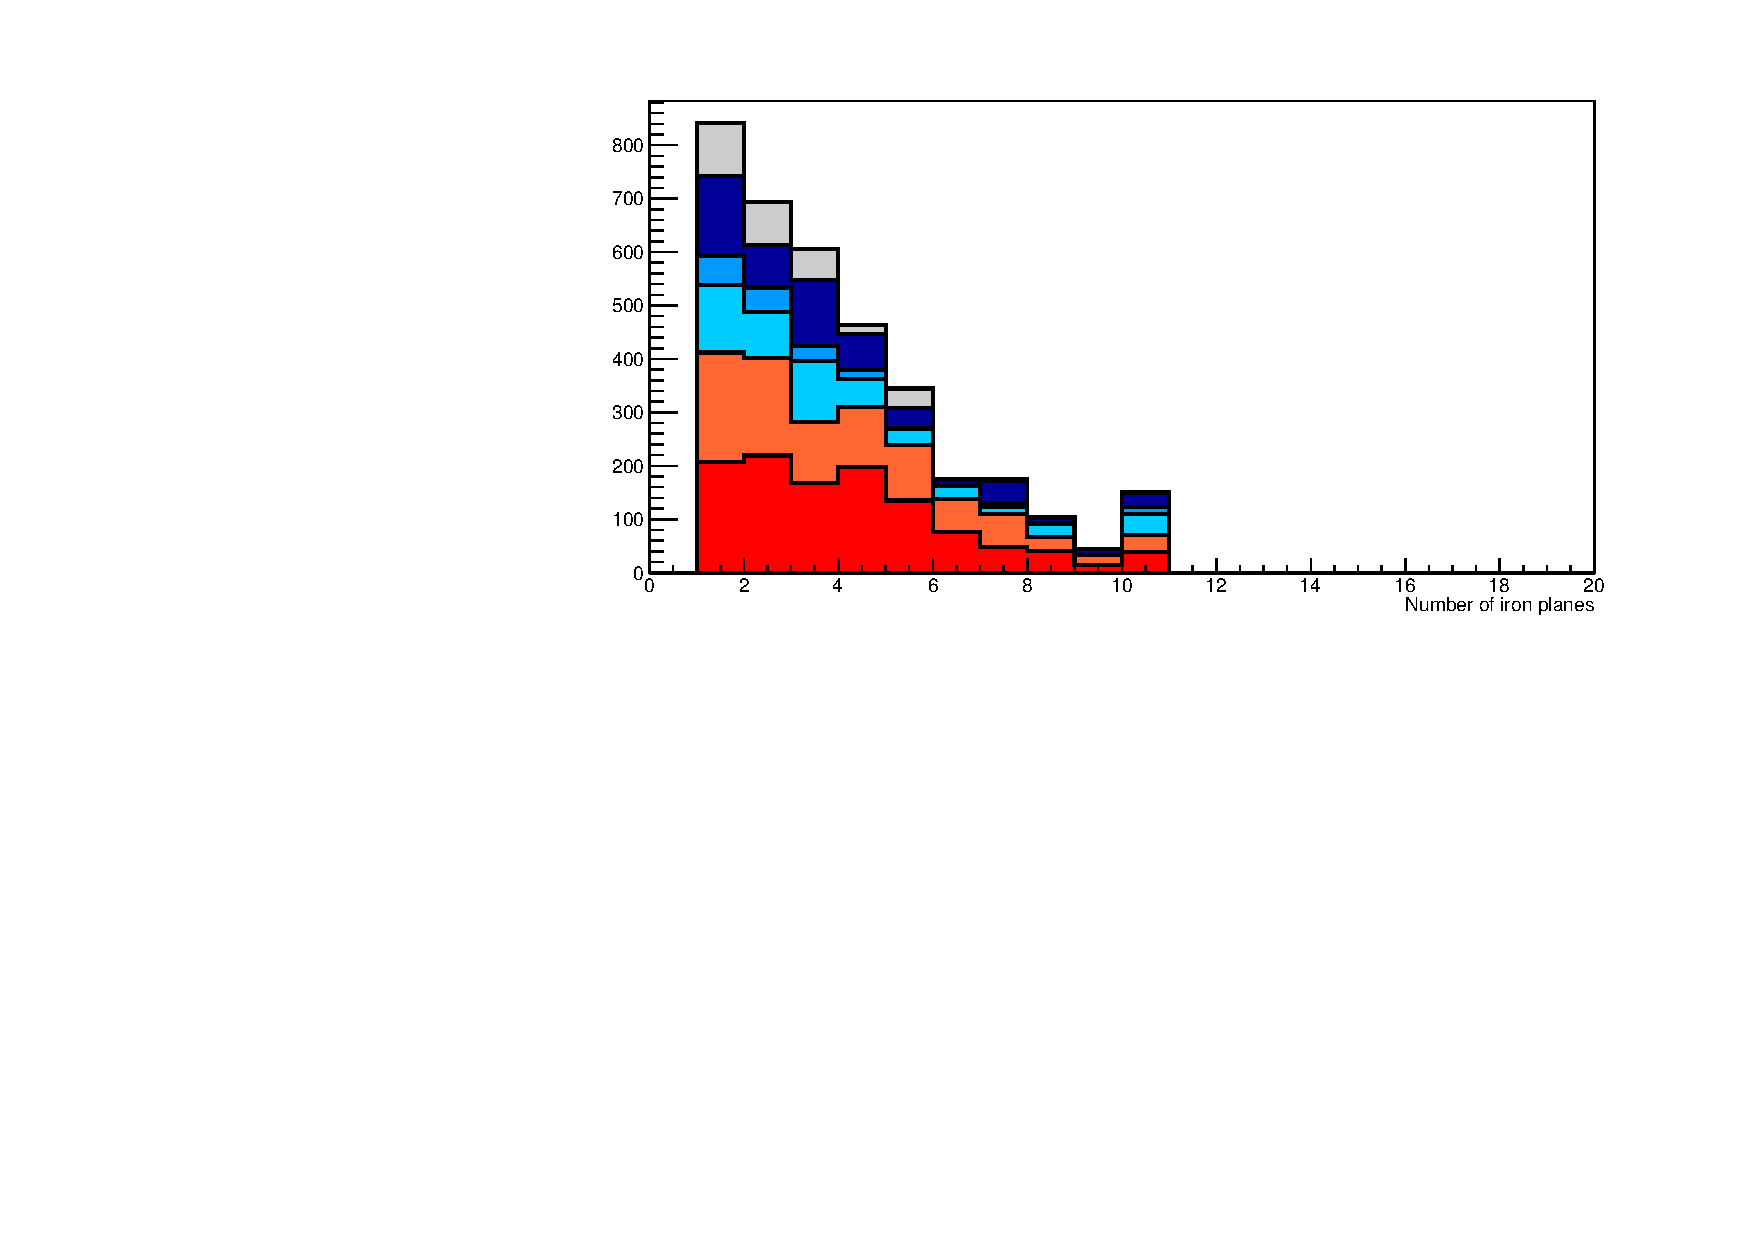
\includegraphics[width=0.8\linewidth, angle=270]{fig/FHCMuonPenetration_SideMRD_StoppedOrThroughGoing.pdf}
    \end{subfigure}
  \begin{subfigure}{0.48\textwidth}
      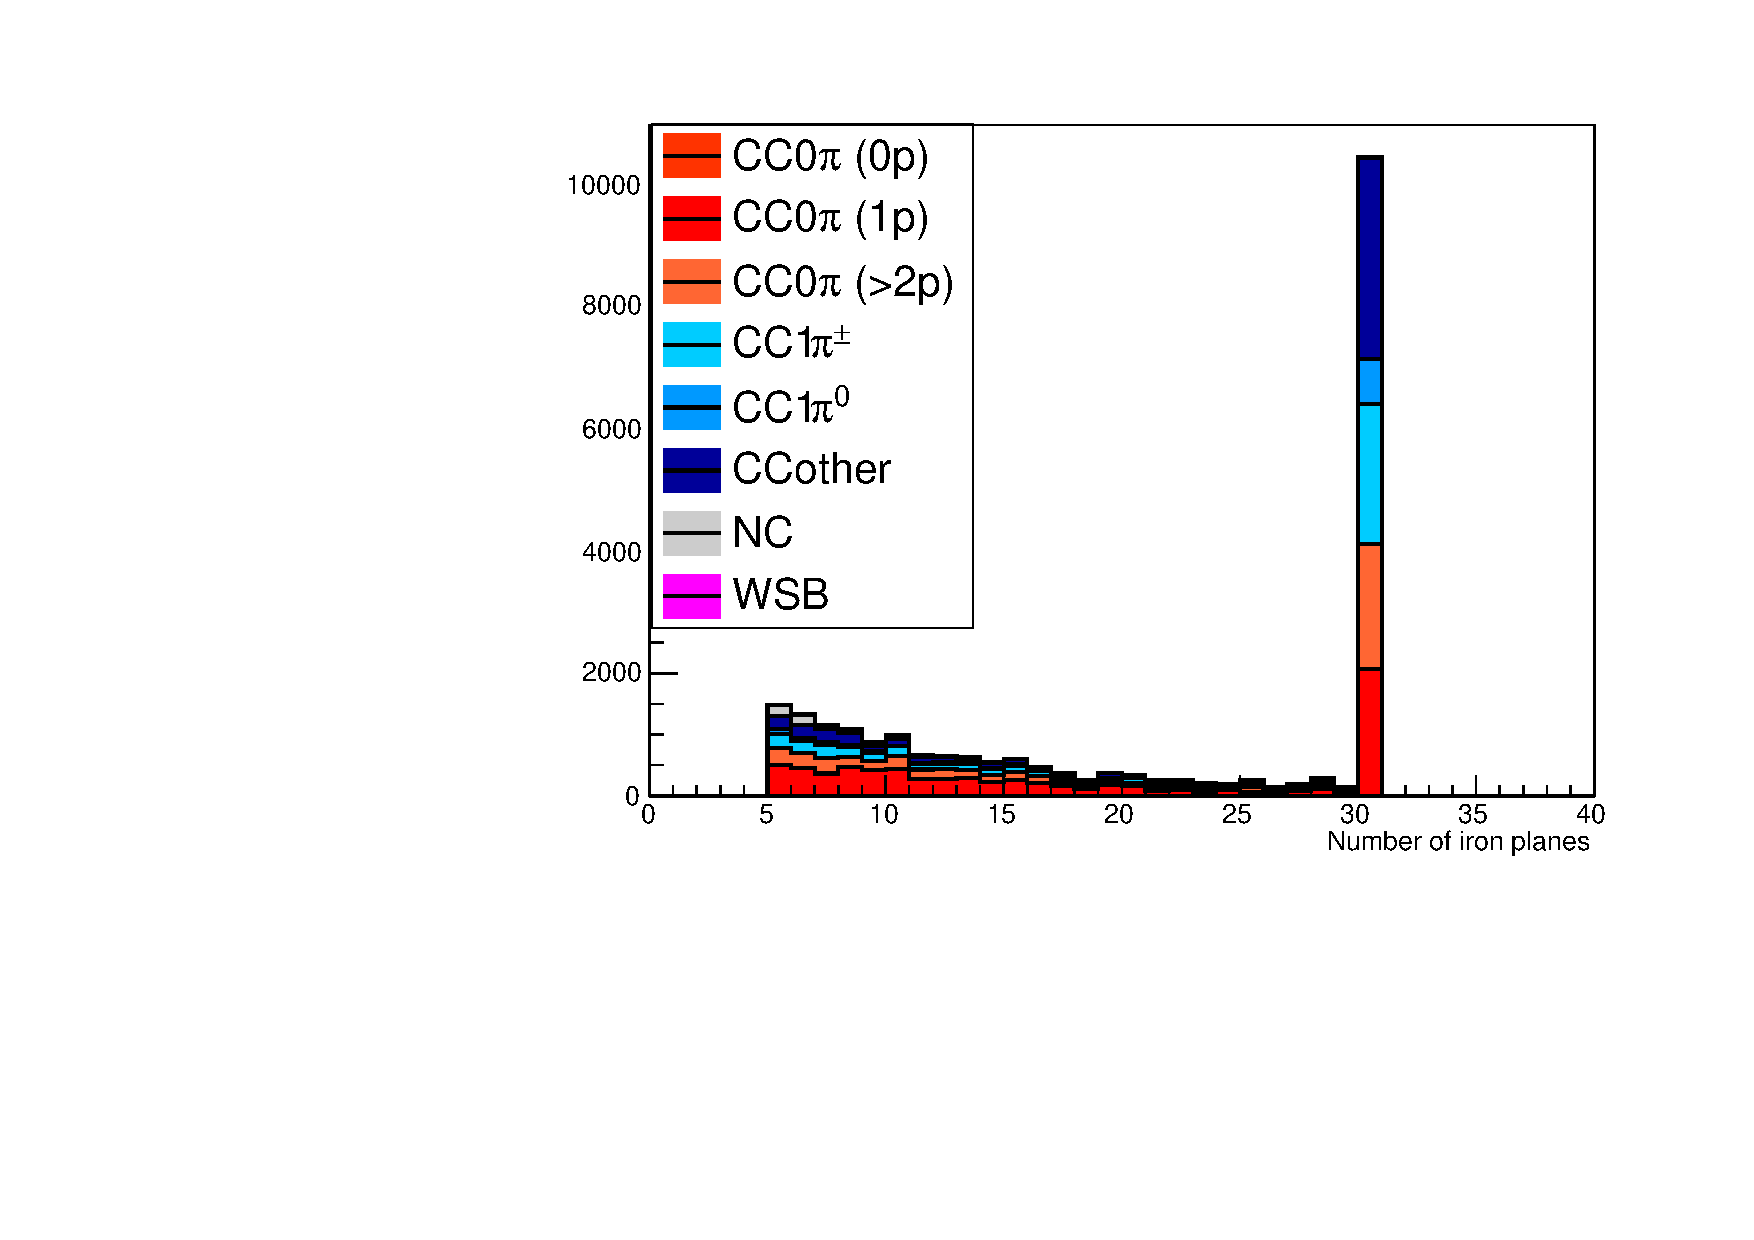
\includegraphics[width=0.8\linewidth, angle=270]{fig/FHCMuonPenetration_DownstreamMRD_StoppedOrThroughGoing.pdf}
    \end{subfigure}    
    \end{center}
  \caption{
Iron plane numbers in Side-MRD (left) and Baby-MIND (right) corresponding to the end points of the longest tracks in the selected events in the neutrino-mode.
%Blue and red hist. are events from water and scintillators in the Wagasci modules, green hist. are events from the experimental hall, and yellow hist. are events from the Side-MRD modules and the Baby-MIND.
}
\label{fig:endpoint_longest_track_neutrino}
\end{figure}

\begin{figure}[tbh]
  \begin{center}
   \begin{subfigure}{0.48\textwidth}
     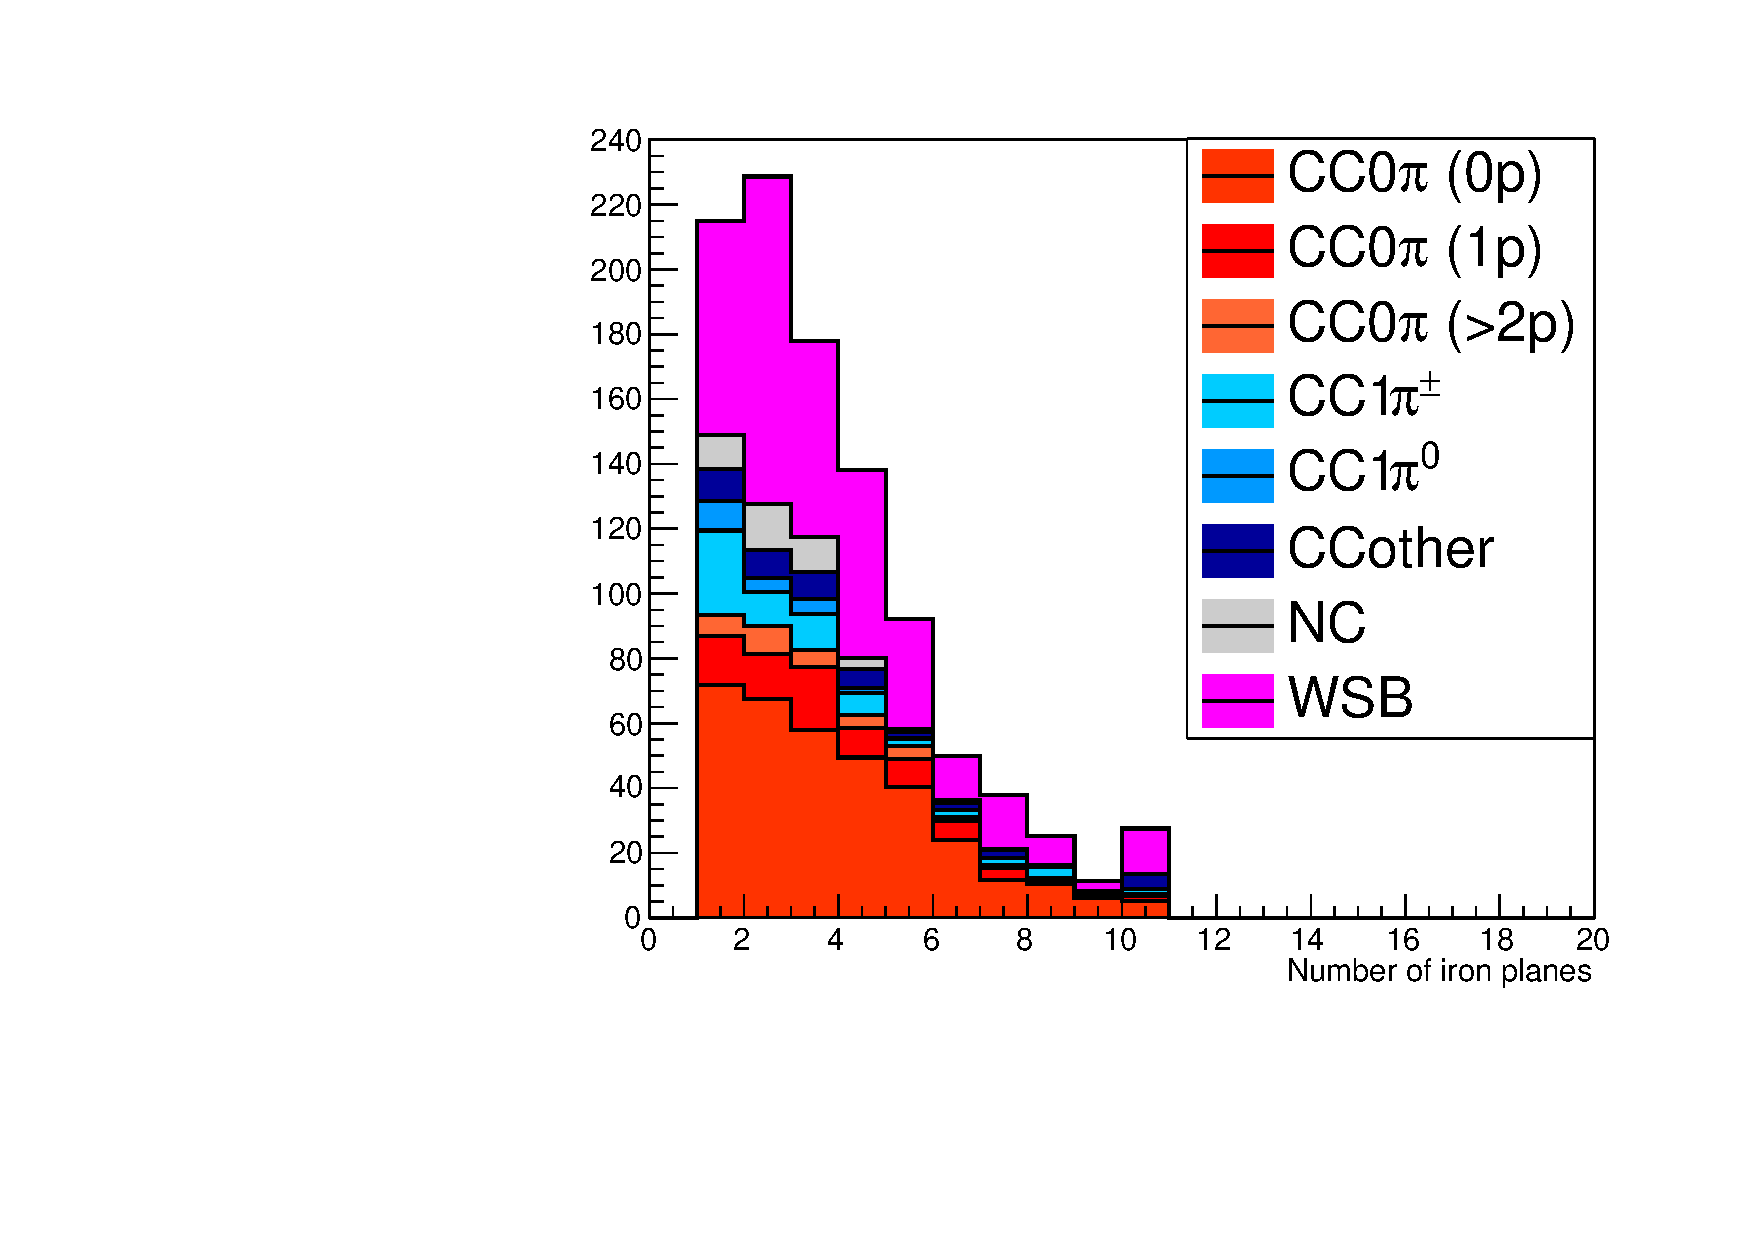
\includegraphics[width=0.8\linewidth, angle=270]{fig/RHCMuonPenetration_SideMRD_StoppedOrThroughGoing.pdf}
    \end{subfigure}
  \begin{subfigure}{0.48\textwidth}
      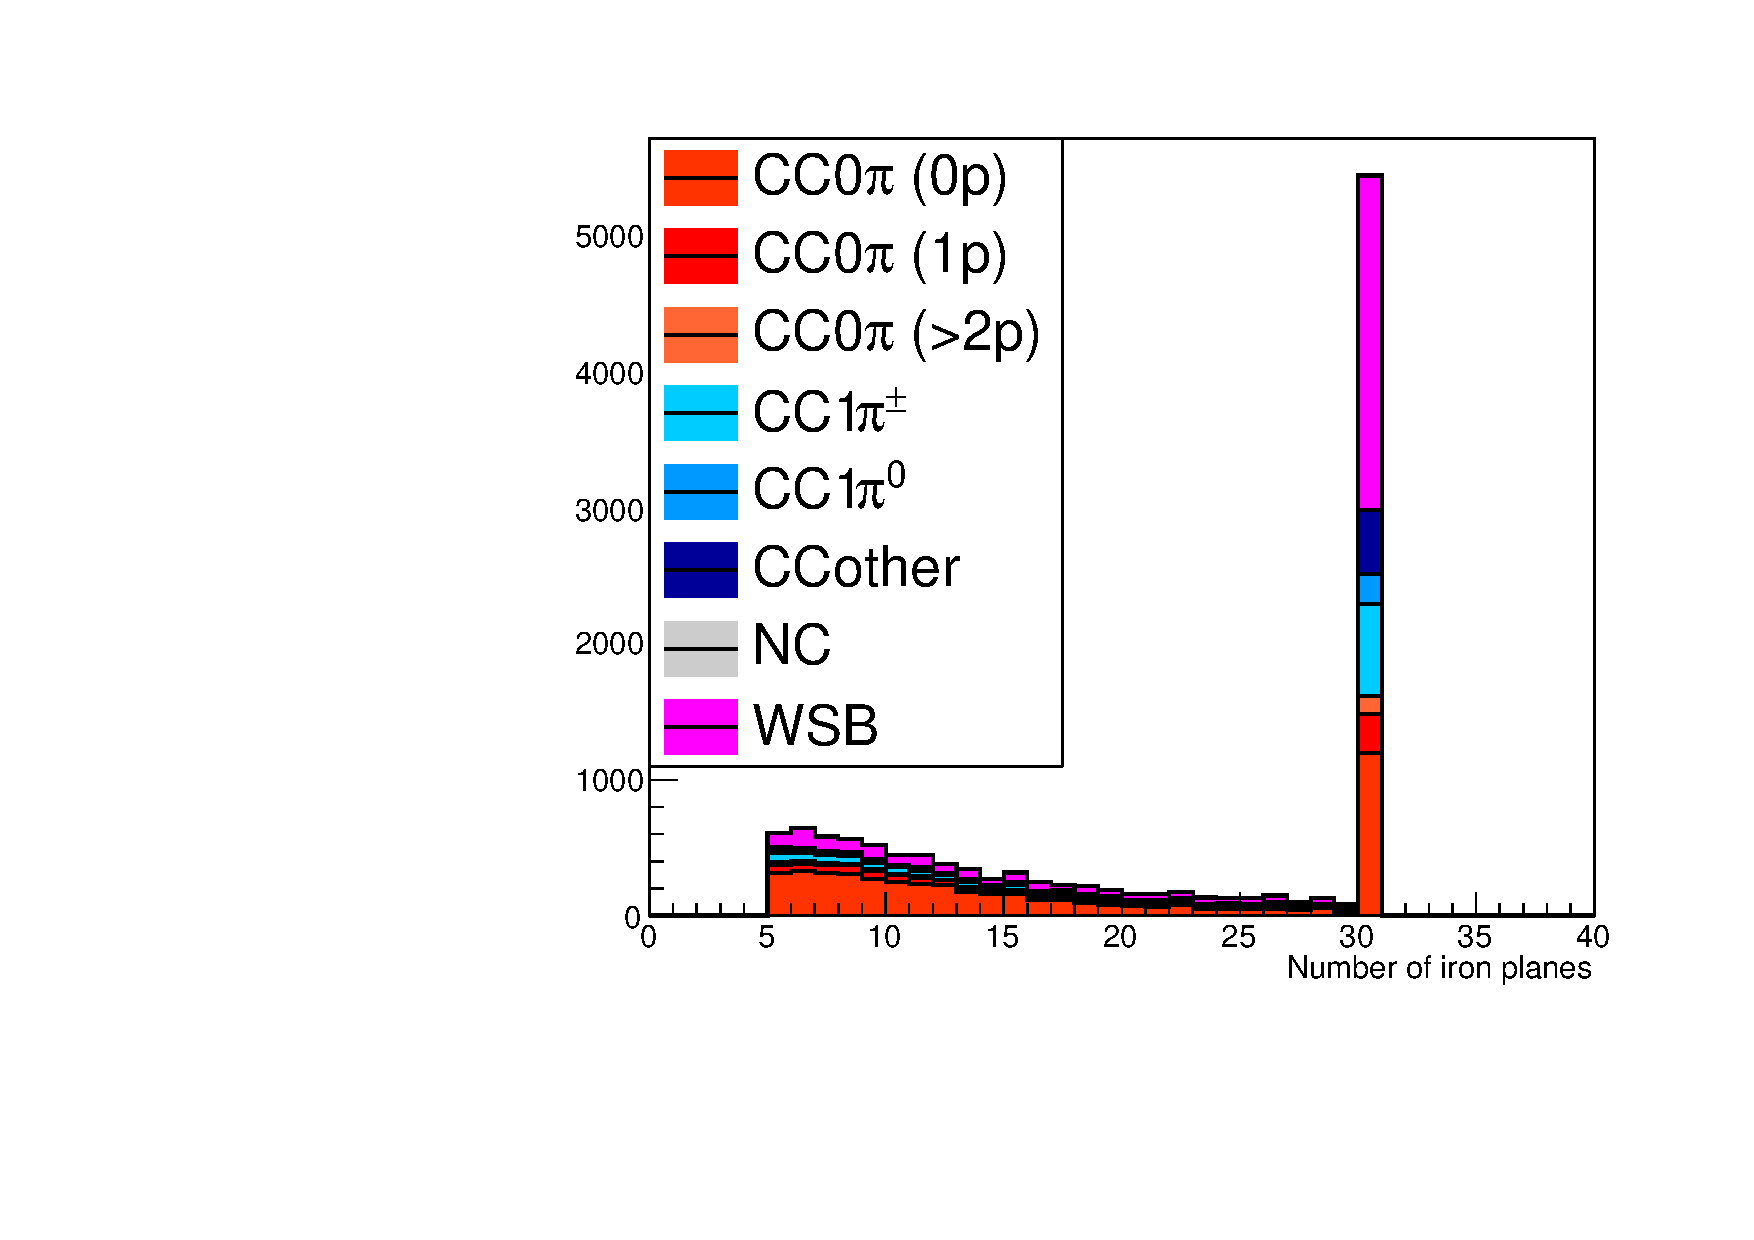
\includegraphics[width=0.8\linewidth, angle=270]{fig/RHCMuonPenetration_DownstreamMRD_StoppedOrThroughGoing.pdf}
    \end{subfigure}    
    \end{center}
  \caption{
Iron plane numbers in Side-MRD (left) and Baby-MIND (right) corresponding to the end points of the longest tracks in the selected events in the antineutrino-mode.
% Blue and red hist. are events from water and scintillators in the Wagasci modules, green hist. are events from the experimental hall, and yellow hist. are events from the Side-MRD modules and the Baby-MIND.
}
\label{fig:endpoint_longest_track_antineutrino}
\end{figure}


%Table \ref{tab:longest_track_particle} shows particles which produce the longest tracks in the selected events, and the fraction of muons is 85.6\%.
%
%\begin{table}[htb]
% \begin{center}
%   \caption{Particles which produce the longest tracks in the selected events.}
 %   \begin{tabular}{cc} \hline
 %     particles & fraction \\ \hline
 %     $\mu$ & 85.6\% \\
 %     $\pi^{+},\ \pi^{-}$ & 4.8\% \\
 %     p & 4.3\% \\
 %     e$^{+}$, e$^{-}$ & 4.5\% \\
 %     \hline
 %   \end{tabular}
 %   \label{tab:longest_track_particle}
 % \end{center}
% \end{table}

% Figure \ref{fig:eff_muon_angle_momentum_neutrino} shows detection efficiencies of muon tracks in the selected events as a function of muon's true angle and true momentum.
% The efficiency in the large angle region is low because Side-MRD modules only cover sides of the Wagasci modules.
% The efficiency in the low momentum region is also low because more than two hits  are required to reconstruct the track in the Wagasci detector.

% \begin{figure}[tbh]
%  \begin{center}
%   \begin{subfigure}{0.48\textwidth}
%     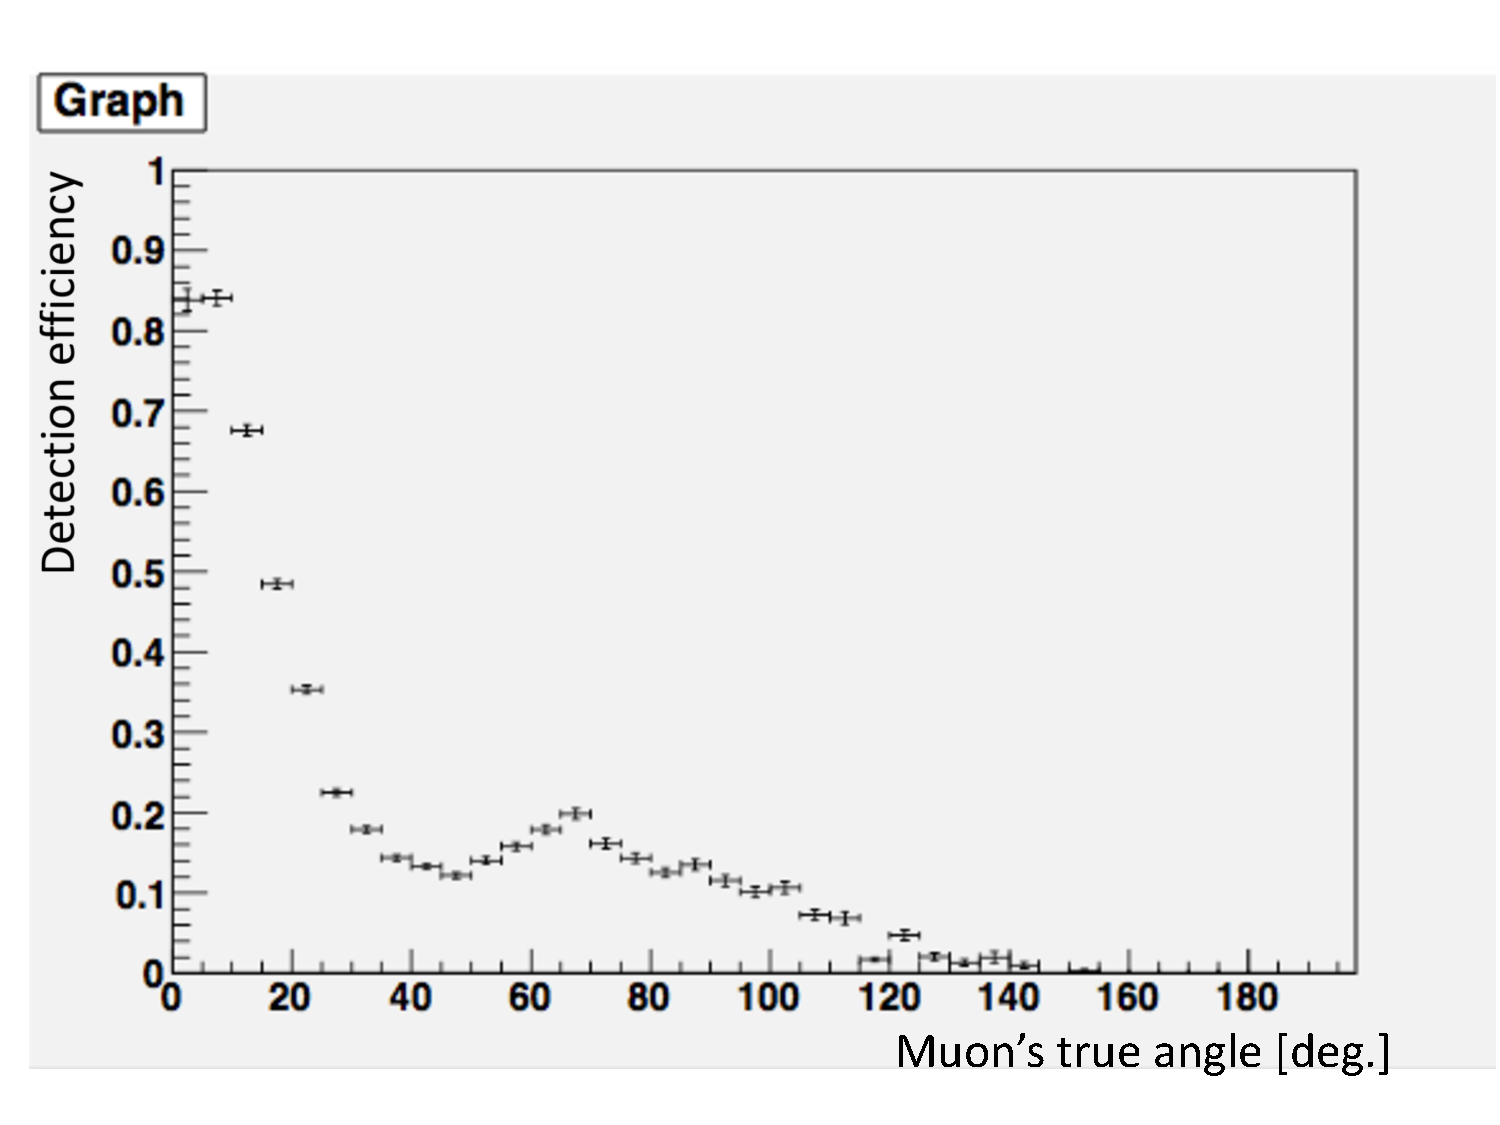
\includegraphics[width=\linewidth]{fig/eff_muon_angle_neutrino.pdf}
%    \end{subfigure}
%  \begin{subfigure}{0.48\textwidth}
%      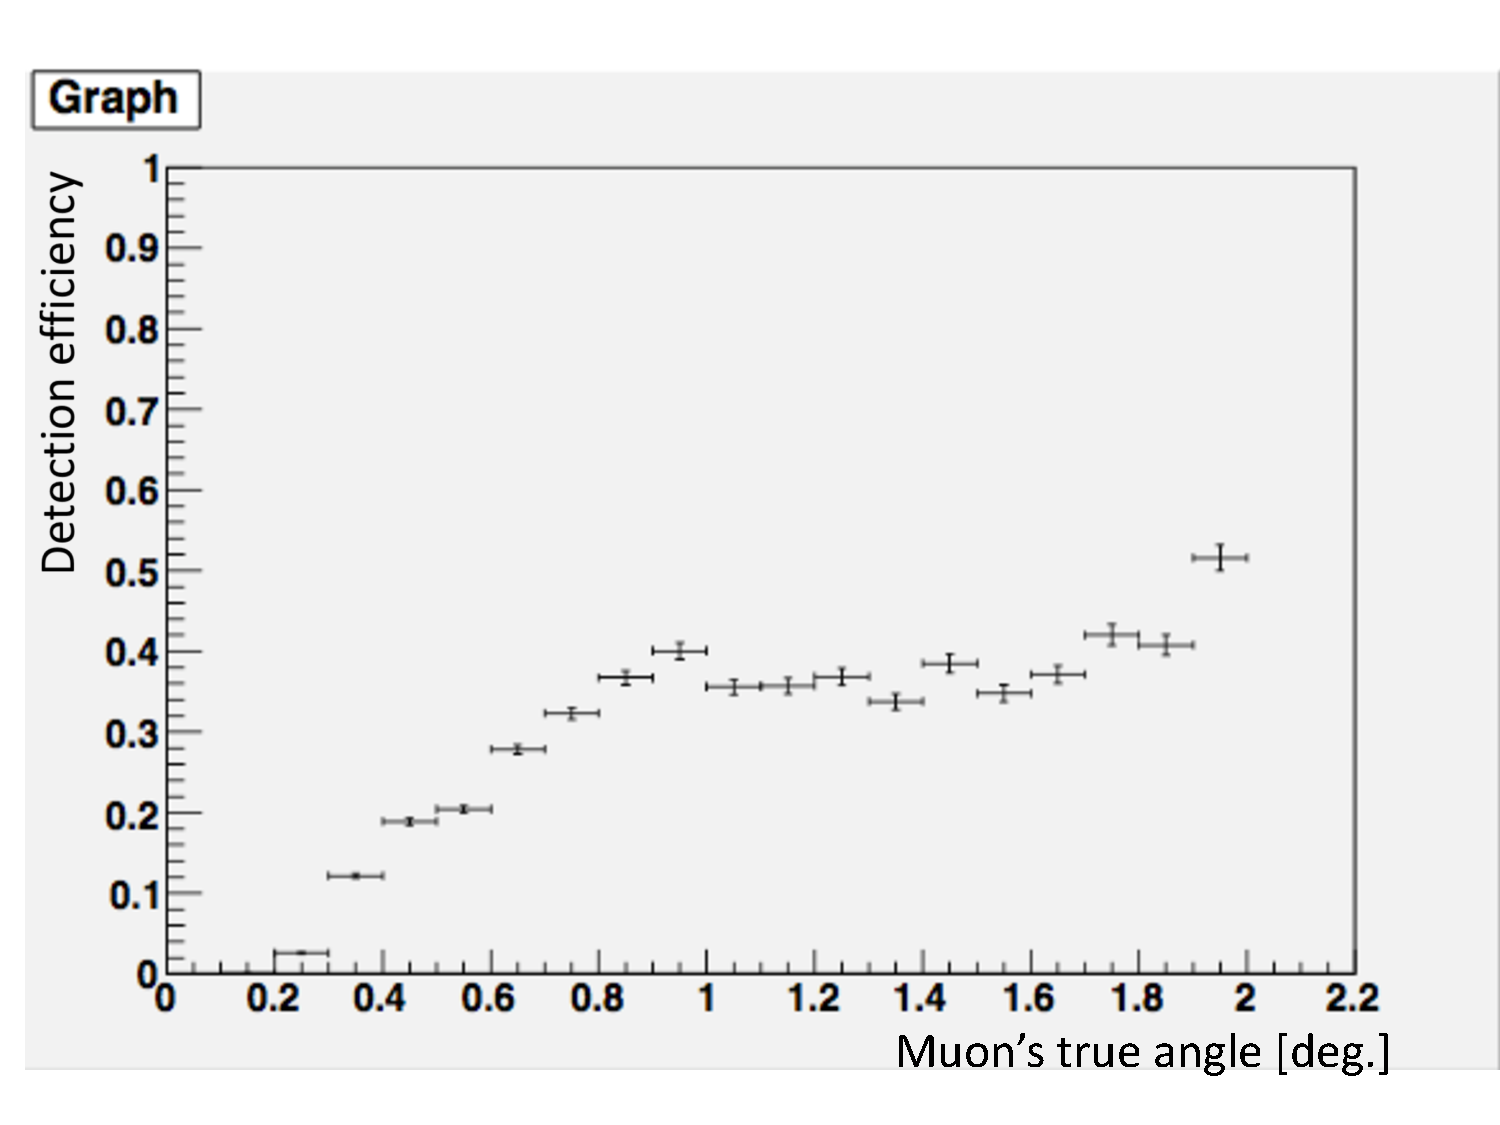
\includegraphics[width=\linewidth]{fig/eff_muon_momentum_neutrino.pdf}
%    \end{subfigure}    
%    \end{center}
%  \caption{
%Detection efficiencies of muon tracks in the selected events as a function of muon's true angle (left) and true momentum (right).
%}
%\label{fig:eff_muon_angle_momentum_neutrino}
%\end{figure}


\subsection{Cross section measurements on water}
In the water target events, the background from interaction with scintillators has to be subtracted by using the measurement of the hydrocarbon target.


\subsubsection{Charged current cross section measurement}


